%--------------------------------------------------------------
% thesis.tex 
%--------------------------------------------------------------
% Corso di Laurea in Informatica 
% http://if.dsi.unifi.it/
% @Facolt\`a di Scienze Matematiche, Fisiche e Naturali
% @Universit\`a degli Studi di Firenze
%--------------------------------------------------------------
% - template for the main file of Informatica@Unifi Thesis 
% - based on Classic Thesis Style Copyright (C) 2008 
%   Andr\'e Miede http://www.miede.de   
%--------------------------------------------------------------
\documentclass[twoside,openright,titlepage,fleqn,
headinclude,12pt,a4paper,BCOR5mm,footinclude]{scrbook}
%--------------------------------------------------------------
\newcommand{\myItalianTitle}{Esprimere in FACPL politiche di controllo degli accessi basate sul comportamento passato\xspace}
\newcommand{\myEnglishTitle}{Expressing access control policies based on past behavior in FACPL\xspace}
% use the right myDegree option
\newcommand{\myDegree}{Corso di Laurea in Informatica\xspace}
%\newcommand{\myDegree}{
	%Corso di Laurea Specialistica in Scienze e Tecnologie 
	%dell'Informazione\xspace}
	\newcommand{\myName}{Federico Schipani\xspace}
	\newcommand{\myProf}{Rosario Pugliese\xspace}
	\newcommand{\myOtherProf}{Andrea Margheri\xspace}
	\newcommand{\myFaculty}{
	Scuola di Scienze Matematiche, Fisiche e Naturali\xspace}
	\newcommand{\myUni}{\protect{
	Universit\`a degli Studi di Firenze}\xspace}
	\newcommand{\myLocation}{Firenze\xspace}
	\newcommand{\myTime}{Anno Accademico 2014-2015\xspace}
	\newcommand{\myVersion}{Version 0.1\xspace}
%--------------------------------------------------------------
\usepackage[italian]{babel}
\usepackage[utf8x]{inputenc} 
\usepackage[T1]{fontenc} 
\usepackage[square,numbers]{natbib} 
\usepackage[fleqn]{amsmath}  
\usepackage{ellipsis}
\usepackage{listings}
\usepackage{subfig}
\usepackage[figurename=Figura]{caption}
\usepackage{appendix}
\usepackage{siunitx}
\usepackage{float}
%--------------------------------------------------------------
\usepackage{dia-classicthesis-ldpkg}
%--------------------------------------------------------------
% Options for classicthesis.sty:
% tocaligned eulerchapternumbers drafting linedheaders 
% listsseparated subfig nochapters beramono eulermath parts 
% minionpro pdfspacing
\usepackage[eulerchapternumbers,linedheaders,subfig,beramono,eulermath,
parts]{classicthesis}
%--------------------------------------------------------------
\newlength{\abcd} % for ab..z string length calculation
% how all the floats will be aligned
\newcommand{\myfloatalign}{\centering} 
\setlength{\extrarowheight}{3pt} % increase table row height
\captionsetup{format=hang,font=small}



%--------------------------------------------------------------
% Comandi personali
%--------------------------------------------------------------
\usepackage{verbatimbox}
\usepackage[pdftex]{graphicx}
\usepackage{rotating}
\usepackage{acronym}
\captionsetup[figure]{labelformat=simple, labelsep=colon}
\graphicspath{{Chapters/Image/}}
\newcommand{\MyFigure}[3]{
	\begin{figure}[H]

		\centering
		\includegraphics[width=#3\linewidth]{#1}
		\caption{ #2 }\label{fig:#1}
		
	\end{figure}
}

\newcommand{\MyFig}[4]{
	\begin{figure}[#4]

		\centering
		\includegraphics[width=#3\linewidth]{#1}
		\caption{ #2 }\label{fig:#1}
		
	\end{figure}
}

\newcommand{\statusattribute}{\textit{Status Attribute}}
\newcommand{\status}{\textit{Status}}


\newcommand{\sr}[1]{#1}

\newcommand{\define}{\triangleq}



\newcommand{\modif}[1]{{\color{red}#1}}

%---------------------------------------
%ACRONYM
%---------------------------------------
\newcommand{\xacml}{\ac{XACML}}
\newcommand{\facpl}{\ac{FACPL}}
\newcommand{\pbac}{\ac{PBAC}}
\newcommand{\rbac}{\ac{RBAC}}

\newcommand{\pdp}{\ac{PDP}}
\newcommand{\pep}{\ac{PEP}}
\newcommand{\pap}{\ac{PAP}}
\newcommand{\pip}{\ac{PIP}}
\newcommand{\pr}{\ac{PR}}

\newcommand{\dsl}{\ac{DSL}}
\newcommand{\ide}{\ac{IDE}}

%%%%%%%%%%%%%%%%%%%%%%%%%%%%%
%SYNTAX
%%%%%%%%%%%%%%%%%%%%%%%%%%%%%
%-----------------------------------
%Algorithm
%-----------------------------------

\newcommand{\denyOver}{\x{d}\textrm{-}\x{over}}
\newcommand{\permitOver}{\x{p}\textrm{-}\x{over}}
\newcommand{\permitUnless}{\x{p}\textrm{-}\x{unless}\textrm{-}\x{d}}
\newcommand{\denyUnless}{\x{d}\textrm{-}\x{unless}\textrm{-}\x{p}}
\newcommand{\onlyOneApp}{\x{one}\textrm{-}\x{app}}
\newcommand{\firstApp}{\x{first}\textrm{-}\x{app}}
\newcommand{\weakCon}{\x{weak}\textrm{-}\x{con}}
\newcommand{\strongCon}{\x{strong}\textrm{-}\x{con}}


\newcommand{\denyOverO}[1]{\x{d}\textrm{-}\x{over}_{\x{#1}}}
\newcommand{\permitOverO}[1]{\x{p}\textrm{-}\x{over}_{\x{#1}}}
\newcommand{\permitUnlessO}[1]{\x{p}\textrm{-}\x{unless}\textrm{-}\x{d}_{\x{#1}}}
\newcommand{\denyUnlessO}[1]{\x{d}\textrm{-}\x{unless}\textrm{-}\x{p}_{\x{#1}}}
\newcommand{\onlyOneAppO}[1]{\x{one}\textrm{-}\x{app}_{\x{#1}}}
\newcommand{\firstAppO}[1]{\x{first}\textrm{-}\x{app}_{\x{#1}}}
\newcommand{\weakConO}[1]{\x{weak}\textrm{-}\x{con}_{\x{#1}}}
\newcommand{\strongConO}[1]{\x{strong}\textrm{-}\x{con}_{\x{#1}}}

%Obligation Types
\newcommand{\obM}{\modif{\x{M}}}
\newcommand{\obO}{\modif{\x{O}}}


%PEP
\newcommand{\based}{\x{base}}
\newcommand{\debugAlg}{\x{debug}}
\newcommand{\denyBiased}{\x{deny}\textrm{-}\x{biased}}
\newcommand{\permitBiased}{\x{permit}\textrm{-}\x{biased}}

%-------------------------------------
%Syntax formatting, comparison functions, examples
%-------------------------------------

\newcommand{\alice}{\x{Alice}}
\newcommand{\bob}{\x{Bob}}

\newcommand{\polSet}[4]{{\bf{\{}}#1{\,}\x{target:}\,#2 {?}\, \x{policies:}#3^{+} {\,}\x{obl:}#4^{*}\, {\bf{\}}}}
\newcommand{\polSetE}[4]{{\bf{\{}}#1 \, \x{target:}\,#2 \, \x{policies:}#3 \, \x{obl:}#4 \, {\bf{\}}}}
\newcommand{\pol}[4]{{\bf{\langle}}#1{\,}\x{target:}\,#2 {?}{\,}\, \x{rules:}#3^{+} {\,}\x{obl:}#4^{*}{\,}{\bf{\rangle}}}
\newcommand{\polE}[4]{{\bf{\langle}}#1{\,}\x{target:}\,#2 {\,}\, \x{rules:}#3 {\,}\x{obl:}#4 {\,}{\bf{\rangle}}}

\newcommand{\pdpPol}[2]{\{ #1 \,  \, #2 \}}
\newcommand{\obl}[1]{\, PepAction( #1^* ) }

\newcommand{\streq}{\x{equal}}
\newcommand{\exprOp}{\x{eop}}
\newcommand{\exprOperator}{\x{op}}

\newcommand{\attribute}[2]{( #1 , #2 )}

%\newcommand{\mEl}{m}
%\newcommand{\mEval}[2]{#2 \models #1}

\newcommand{\x}[1]{{\sf #1}}


%---------------------------------------
% Separator
%---------------------------------------

\newcommand{\set}[1]{\{#1\}} % brackets for sets
\newcommand{\Sep}{\ \mid\ }

\newcommand{\policySetBegin}{{\bf{\{}}}
\newcommand{\policyBegin}{{\bf{\{}}}
\newcommand{\policySep}{\,\bf{\ }\,}
\newcommand{\policiesBegin}{\x{policies:}\,}
\newcommand{\targetBegin}{\x{target:}\,}
\newcommand{\targetEnd}{\,{\bf{\ }}}
\newcommand{\policiesEnd}{\,{\bf{\ }}}
%\newcommand{\rulesBegin}{\x{rules:}\,}
%\newcommand{\rulesEnd}{\,{\bf{\ }}}
\newcommand{\policyEnd}{{\bf{\}}}}
\newcommand{\policySetEnd}{{\bf{\}}}}
%\newcommand{\conditionBegin}{\x{condition:}\,}
%\newcommand{\conditionEnd}{\,{\bf{\ }}}
\newcommand{\oblsBegin}{\x{obl:}\,}
\newcommand{\oblsEnd}{\bf{\ }\,}
\newcommand{\oblBegin}{{\bf{[}}}
\newcommand{\oblEnd}{{\bf{]}}}

\newcommand{\match}[3]{#1{\bf(}#2{\bf,}#3{\bf)}}
\newcommand{\ruleOpt}[1]{{\bf{(}}#1{\bf{)}}}
\newcommand{\oblOpt}[1]{{\bf{(}}#1{\bf{)}}}

\newcommand*\lfrac[2]{{}_{#1}\!\backslash\!^{#2}} % table combining algorithm

%------------------------------
%Decisions & values
%------------------------------
\newcommand{\permit}{\x{permit}}
\newcommand{\deny}{\x{deny}}
\newcommand{\notApp}{\x{not}\textrm{-}\x{app}}
\newcommand{\indet}{\x{indet}}
\newcommand{\excpt}{\perp}
\newcommand{\err}{\x{error}}

\newcommand{\indetD}{\x{indetD}}
\newcommand{\indetP}{\x{indetP}}
\newcommand{\indetDP}{\x{indetDP}}

\newcommand{\true}{\x{true}} 
\newcommand{\false}{\x{false}} 

%%%%%%%%%%%%%%%%%%%%%%%
%SEMANTICS
%%%%%%%%%%%%%%%%%%%%%%%

%Auxiliary Semantic Functions and notations
\newcommand{\pepSemR}[1]{(\!( #1 )\!)}
\newcommand{\concat}{{\bullet}}
\newcommand{\subobeff}[2]{#1\!\!\mid_{#2}} %sub sequence of obligations

%Name of Semantic Function
\newcommand{\denSemF}[1]{\mathcal{ #1 }}

%Semantic Brakets
%\newcommand{\denSem}[2]{[\![ #1 ]\!]_{#2}}
\newcommand{\denSem}[2]{[\![ #1 ]\!] #2}

%Named Semantics Functions
\newcommand{\policySem}[2]{\denSemF{P}\denSem{#1}{#2}}
\newcommand{\algSem}[2]{\denSemF{A}\denSem{#1}{#2}}
\newcommand{\exprSem}[2]{\denSemF{E}\denSem{#1}{#2}}
\newcommand{\oblSem}[2]{\denSemF{O}\denSem{#1}{#2}}
\newcommand{\oblSemS}[2]{\denSemF{OS}\denSem{#1}{#2}}
\newcommand{\pdpSem}[2]{\denSemF{P}dp\denSem{#1}{#2}}
\newcommand{\pepSem}[2]{\denSemF{E}A\denSem{#1}{#2}}
\newcommand{\pasSem}[1]{\denSemF{P}as\denSem{#1}{}}
\newcommand{\reqSemS}[2]{\denSemF{R}\denSem{#1}{#2}}  %two arguments, \name as second argument
\newcommand{\reqSem}[1]{\denSemF{R}\denSem{#1}{}} %used for PAS semantics

%Generic Element of each Syntactic Category
\newcommand{\expr}{\mathit{expr}}
\newcommand{\effect}{\mathit{e}}
\newcommand{\ob}{\mathit{o}}
\newcommand{\obType}{\mathit{t}}
\newcommand{\fo}{\mathit{f\!o}}
\newcommand{\foS}{\mathit{f\!o}^*}
\newcommand{\rSyntax}{\mathit{req}} %element of syntactic category Request
\newcommand{\req}{\mathit{r}} % element of functional representation of Request
\newcommand{\policy}{\mathit{p}}
\newcommand{\algSyntax}{\mathit{a}}
\newcommand{\pdpRes}{\mathit{res}}
\newcommand{\dec}{\mathit{dec}} %decision
\newcommand{\double}{\mathit{d}} %double
\newcommand{\extVal}{\mathit{w}} % Obligations and table of expression semantics
\newcommand{\enfAlg}{\mathit{ea}}
\newcommand{\pdpSyntax}{\mathit{pdp}}
\newcommand{\name}{\mathit{n}}
\newcommand{\val}{\mathit{v}}
\newcommand{\pepAction}{\mathit{pepAct}}

\newcommand{\algNT}{\mathit{Alg}} %used in syntax section
\newcommand{\algName}{\mathsf{alg}} % used in combining algorithms semantic section

%Semantics of Combiing Algorithms
\newcommand{\alg}[1]{\mathsf{alg}_{#1}}
\newcommand{\algD}{\alg{\delta}}
\newcommand{\algOp}{\otimes \mathsf{alg}}
\newcommand{\algOpAlg}[1]{\otimes #1}

\newcommand{\all}{\x{all}}
\newcommand{\greedy}{\x{greedy}}
\newcommand{\isFinal}[2]{\mathit{isFinal}_{#1}({#2})}
\newcommand{\isFinalPred}[1]{\mathit{isFinal}_{#1}}


\renewcommand{\lstlistingname}{Codice}
\renewcommand{\lstlistlistingname}{Lista di Codici}

\definecolor{eclipsePurple}{RGB}{127,0,85}
\definecolor{dkgreen}{rgb}{0,.6,0}
\definecolor{brightpink}{rgb}{1.0, 0.0, 0.5}
\definecolor{burgundy}{rgb}{0.5, 0.0, 0.13}
\lstdefinelanguage{Xtend}{
 morekeywords={cached,case,default,extension,false,import,JAVA,WORKFLOWSLOT,let,new,null,private,create,switch,this,true,reexport,around,if,then,else,context},
 keywordstyle=[2]{\textbf},
 morecomment=[l]{//}, 
 morecomment=[s]{/*}{*/}, 
 morestring=[b]",
 tabsize=4}
 \lstdefinelanguage{Xtext}{
 morekeywords={grammar, with, hidden, generate, as, import, returns, current, terminal, enum},
 keywordstyle=[2]{\textbf},
 morecomment=[l]{//}, 
 morecomment=[s]{/*}{*/}, 
 morestring=[b]",
 tabsize=4}
\lstdefinelanguage{FACPL} {
  % list of keywords
	keywords = [1] {
		deny-biased, permit-biased, deny-unless-permit, unless, biased
	},
  	morekeywords = [2] {
		target, policies, obl, rules
	},
	keywords = [3] {
		addStatus, subStatus, equal, flagstatus,
		less-than, greater-than, sumDate, setString
	},
	keywords = [4] { 
		Policy, PolicySet, Rule, Request
	},
	keywords = [5] {
		permit, deny
	},
  %style
	keywordstyle = [1]{		
		\color{dkgreen}
	},
	keywordstyle = [2]{
		\color{burgundy}\bfseries
	},
	keywordstyle = [3]{
		\color{dkgreen}
	},
	keywordstyle = [4]{
		\color{orange}\bfseries
	},
	keywordstyle = [5]{
		\color{brightpink}\bfseries
	},
	sensitive=false, 
	morecomment=[l]{//}, 
	morecomment=[s]{/*}{*/}, 
	morestring=[b]",
	morestring=[b]',
	stringstyle=\color{blue}\ttfamily
}
\definecolor{mygray}{rgb}{0.5,0.5,0.5}
\lstdefinestyle{javigno}{
	frame=tb,
	language=Java,
	aboveskip=3mm,
	belowskip=3mm,
	showstringspaces=false,
	columns=flexible,
	basicstyle={\small\ttfamily},
	numbers=left,
	numberstyle=\tiny\color{mygray},
	numbersep=5pt,
	stepnumber=2,
	breaklines=true,
	breakatwhitespace=true,
	tabsize=3
}

\newcommand{\myIjava}[5]
	{
		\lstinputlisting[language = Java, style = javigno, firstnumber = #3, firstline = #3, lastline = #4, caption = {#2}\label{lst:#5}]{./Source/Java/#1}
	}
\newcommand{\myjava}[2]
	{
		\lstinputlisting[language = Java, style = javigno, caption = {#2}\label{lst:#1}]{./Source/Java/#1}
	}

%--------------------------------------------------------------
% Layout setting
%--------------------------------------------------------------
\usepackage{geometry}
\geometry{
a4paper,
ignoremp,
bindingoffset = 1cm, 
textwidth     = 13.5cm,
textheight    = 21.5cm,
	lmargin       = 3.5cm, % left margin
	tmargin       = 4cm    % top margin 
	}

	\lstset{
	frame=tb,
	language=Java,
	aboveskip=3mm,
	belowskip=3mm,
	showstringspaces=false,
	columns=flexible,
	basicstyle={\footnotesize\ttfamily},
	numbers=left,
	stepnumber = 2,
	breaklines=true,
	breakatwhitespace=true,
	tabsize=2
	}
%--------------------------------------------------------------
\begin{document}
\frenchspacing
\raggedbottom
\pagenumbering{roman}
\pagestyle{plain}
%--------------------------------------------------------------
% Frontmatter
%--------------------------------------------------------------
%--------------------------------------------------------------
% titlepage.tex (use thesis.tex as main file)
%--------------------------------------------------------------
\begin{titlepage}
	\begin{center}
   	\large
      \hfill
      \vfill
      \begingroup
         
\includegraphics[scale=0.15]{logo/LOGO}\\
%			\spacedallcaps{\myUni} \\ 
			\myFaculty \\
			\myDegree \\ 
			\vspace{0.5cm}
         \vspace{0.5cm}    
         Tesi di Laurea    
      \endgroup 
      \vfill 
      \begingroup
      	\color{Maroon}\spacedallcaps{\myItalianTitle} \\ $\ $\\
      	\spacedallcaps{\myEnglishTitle} \\ 	
	\bigskip
      \endgroup
      \spacedlowsmallcaps{\myName}
      \vfill 
      \vfill
      Relatore: \emph{Rosario Pugliese}\\
      Correlatore: \emph{Andrea Margheri}\\
      \vfill
      \vfill
      \myTime
      \vfill                      
	\end{center}        
\end{titlepage}   
%--------------------------------------------------------------
% back titlepage
%--------------------------------------------------------------
   \newpage
	\thispagestyle{empty}
	\hfill
	\vfill
	\noindent\myName: 
	\textit{\myItalianTitle,} 
	\myDegree, \textcopyright\ \myTime
%--------------------------------------------------------------
% back titlepage end
%--------------------------------------------------------------
\pagestyle{scrheadings}
%--------------------------------------------------------------
% Mainmatter
%--------------------------------------------------------------
\pagenumbering{arabic}
% use \cleardoublepage here to avoid problems with pdfbookmark
%\include{intro} % use \myChapter command instead of \chapter
\tableofcontents
\listoffigures
\lstlistoflistings	
\cleardoublepage
\thispagestyle{empty}
\begin{flushright}
\null\vspace{\stretch {1}}
\emph{Ezechiele 25:17. “Il cammino dell'uomo timorato è minacciato da ogni parte dalle iniquità degli esseri egoisti e dalla tirannia degli uomini malvagi. Benedetto sia colui che nel nome della carità e della buona volontà conduce i deboli attraverso la valle delle tenebre, perché egli è in verità il pastore di suo fratello e il ricercatore dei figli smarriti. E la mia giustizia calerà sopra di loro con grandissima vendetta e furiosissimo sdegno su coloro che si proveranno ad ammorbare e infine a distruggere i miei fratelli. E tu saprai che il mio nome è quello del Signore quando farò calare la mia vendetta sopra di te.” \break --- Jules Winnfield [Voce di Luca Ward]} \vspace{\stretch{2}}\null \\
\emph{"Stay hungry, stay hungry" \break --- Paolo Bitta, l'uomo chiamato contratto} \vspace{\stretch{2}}\null
\end{flushright}
\cleardoublepage
\nocite{*}

\myChapter{Introduzione}
FACPL è un linguaggio basato su XACML, e supportato da una libreria scritta in Java, ma con una sintassi molto più semplice e concisa che permette di formalizzare in modo facile, non ambiguo e rapido politiche di \textit{access control}. Però questo linguaggio non godeva di caratteristiche per consentire di fare richieste ed ottenere risposte valutando anche il comportamento passato, quindi l'obiettivo di questa tesi è stato estendere FAPCL in modo da implementare nuove e fondamentali funzionalità che permette di sfruttare questo un nuovo chiamato \textit{Usage Control}. \\ \par
La questione sul controllo agli accessi è un problema molto rilevante a cui si è provato a trovare una soluzione in questi ultimi anni. Negli ultimi decenni, a partire dal 1970, sono stati proposti molti modelli come ACL, RBAC, ABAC e PBAC, ognuno ha i suoi punti di forza ed i suoi punti deboli.
ACL è un modello basato su liste di accesso associate ad ogni risorsa che definiscono le regole di accesso, è un modello molto semplice da implementare, ma quando i dati erano eccessivi diventava poco efficiente. Successivamente è stato introdotto un modello basato su ruoli, il quale associava a insiemi di risorse dei ruoli, ovvero dei gruppi di utenti raggruppati secondo una caratteristica comune. Un punto debole di questo modello è la mancata specificità riguardante la definizione delle regole che rende difficile assegnare permessi particolari a singole risorse. A seguire è stato introdotto un modello basato su attributi dove le decisioni vengono prese valutando caretteristiche del richiedente, della risorsa e dell'ambiente in cui è fatta la richiesta. Un difetto di quest'ultimo modello è che non offre una buona scalabilità. Per porre rimedio a questo difetto è stato introdotto un modello basato su politiche, che oggi risulta essere uno dei più utilizzati, e che si basa su politiche, ovvero un insieme di regole su attributi.
Recentemente, Sandhu e Park, hanno introdotto un'estensione di \textit{Access Control} chiamata \textit{Usage Control} le cui caratteristiche sono la possibilità di prendere decisioni durante l'accesso e basandosi sul comportamento passato. Il che lo rende molto adatto ad ambienti come il Web, Cloud o comunque legati in qualche modo alla rete. \\ \par
Il resto della tesi è organizzato in questo modo. Nel capitolo~\ref{cap:accessControl} vengono analizzati in maggior dettaglio tutti i modelli di \textit{Access Control} descritti precedentemente e inoltre viene dedicata una sezione a \textit{Usage Control} dove vengono anche introdotti due esempi che verranno portati avanti durante gli altri capitoli. Nel capitolo~\ref{cap:facpl} è descritto FACPL allo stato precedente alla stesura di questo documento, ovvero quando ancora non era possibile esprimere politiche di accesso basate sul comportamento passato. Alla fine del capitolo verrà anche proposto un esempio e sarà spiegato perché non è possibile prendere decisioni di \textit{Usage Control}. Nel capitolo~\ref{cap:usagecontrolfacpl} viene trattata l'estensione di FACPL ad un livello sintattico e semantico, spiegando quali nuove componenti sono state introdotte e analizzandone il loro significato ed utilizzo in un contesto reale. A fine capitolo sono riproposti in FACPL gli esempi citati in sezione~\ref{sec:usage_control}, scritti usando le nuove estensioni. Nell'ultimo capitolo, il ~\ref{cap:estensione_libreria} invece sono trattati gli argomenti trattati in quello precedente sotto dell'estensione della libreria per l'implementazione delle nuove funzionalità.


\myChapter{Access Control e Usage Control}
\label{cap:accessControl}
I sistemi informatici moderni sono capaci di condividere dati e
risorse computazionali, ed impedire accessi non autorizzati è diventata
una priorità inderogabile.
I motivi che portano a questa decisione possono essere legati alla privacy o alla consistenza dei dati durante una computazione.
Ad esempio, molte informazioni personali possono essere
raccolte durante alcune attività quotidiane, dunque diventa necessario
proteggere questi dati da malintenzionati. Per questo motivo esistono sistemi di Access Control, ovvero dei sistemi
definiti da un insieme di condizioni che permettono di creare una prima
linea difensiva contro accessi indesiderati.


In Sezione~\ref{sec:history} vengono trattati in maggior dettaglio i vari modelli 
di controllo all'accesso proposti negli ultimi decenni, successivamente, nella Sezione~\ref{sec:usage_control} viene analizzato anche un nuovo modello chiamato \textit{Usage Control}. Infine nell'ultima Sezione, la ~\ref{sec:casi_studio}, vengono proposti due case study.
\section{Access Control}
\label{sec:history}



Negli anni sono stati proposti diversi approcci per cercare di definire un
modello efficiente e scalabile. Andremo ora ad eseguire una classificazione
dei modelli di Access Control, seguendo la catalogazione del NIST \cite{NISTACM}.

\begin{itemize}
\item \acf{ACL} è il primo di questi modelli ed è stato proposto intorno al 1970 spinto
dall’avvento dei primi sistemi multi utente.
\item \acf{RBAC} è nato successivamente ad \ac{ACL} e ne modifica alcuni aspetti in modo da rimuovere
molte delle limitazioni di quest’ultimo. 
\item \acf{ABAC} è nato dopo \ac{RBAC} e fornisce un paradigma dinamico che aiuta a sviluppare policy che si adattano all'ambiente. 
\item \acf{PBAC} è molto simile ad \ac{ABAC} ma migliora e standardizza quest ultimo modello.

\end{itemize}

\subsection*{Access Control Lists}
\label{sub:ACL}

\ac{ACL} è il primo modello di controlli agli accessi, è stato introdotto intorno al 1970 grazie all'avvento dei sistemi multi utente allo scopo di limitare l'accesso a file e dati appartenenti a diversi utenti, infatti i primi sistemi ad utilizzare questo modello sono stati sistemi di tipo UNIX. Con la comparsa della multiutenza per sistemi ad uso personale lo standard \ac{ACL} è stato implementato in molte più ambienti come sistemi UNIX-Like e Windows. \par
Il concetto dietro \ac{ACL} è uno dei più semplici, in quanto ogni risorsa del sistema che deve essere controllata ha una sua lista, che ad ogni soggetto associa le azioni che può effettuare sulla risorsa, ed il sistema operativo quando viene fatta richiesta decide in base alla lista se dare il permesso o meno. 


Per esempio in Figura \ref{fig:acl_osx}, si può vedere come \textit{test\_folder} sia la risorsa da controllare, \textit{federicoschipani}, \textit{staff} e \textit{everyone} siano i soggetti e le azioni associate sono, in questo caso, \textit{Read \& Write} al primo soggetto e \textit{Read only} agli altri due.
\MyFig{acl_osx}{\acf{ACL} in OS X}{0.8}{h}


La semplicità di questo modello non richiede grandi infrastrutture sottostanti, la  sua implementazione dal punto di vista applicativo risulta abbastanza semplice attraverso l'uso di linguaggi ad alto livello come Python o Java, poiché le strutture che servono per implementare questo standard sono già definite.
Nonostante negli anni sono stati sviluppati modelli più complessi, come \ac{ABAC}, \ac{PBAC} e \ac{RBAC}, il sistema descritto in questa sezione viene comunque usato nei sistemi operativi recenti. Come si può vedere in Figura \ref{fig:acl_osx} OS X sfrutta questo standard per la gestione dei permessi sul filesystem. \par
Un aspetto negativo si manifesta quando si trattano grandi quantità di risorse. Ogni volta che viene richiesto l'accesso ad una risorsa da parte di un entità, utente o applicazione che sia, è necessario verificare nella lista associata, il che lo rende abbastanza oneroso dal punto di vista computazionale. \par
Un altro lato negativo emerge quando bisogna effettuare modifiche ai permessi di una determinata risorsa, in quanto è necessario andare ad operare sulla lista di quest'ultima, il che rende questo compito incline ad errori ed oneroso dal punto di vista del tempo.


\subsection*{Role-based Access Control} % (fold)
\label{sub:role_based_access_control}

\ac{RBAC} è l'evoluzione di \ac{ACL}, in quanto tende a correggerne alcuni difetti come la limitata scalabilità. \par
A differenza di \ac{ACL} è presente il concetto il ruolo del richiedente, ovvero un titolo che definisce un livello di autorità, che raggrupperà diversi utenti in una categoria. 
\ac{RBAC} attraverso questa nuova caratteristica riesce a porre rimedio ai difetti di \ac{ACL} in quanto
questo tipo di gestione offre il vantaggio di facilitare l'assegnazione dei permessi, poiché per ogni risorsa non si devono più gestire tutti i singoli utenti, ma basta gestire i permessi associati a queste nuove categorie. 


Un utente può anche far parte di più gruppi, per esempio un contabile di un azienda può far parte del gruppo \textit{impiegati} e \textit{contabili} in modo da permettergli l'accesso sia ai documenti riservati ai soli impiegati che quelli riservati ai soli contabili.
Come si può vedere in Figura \ref{fig:group2} il concetto di gruppo è implementato nei sistemi operativi moderni, in particolare in OS X, Windows e sistemi UNIX-Like.

\MyFig{group2}{Gruppo in OS X}{0.9}{h}
\ac{RBAC} però ha i suoi difetti, uno dei più evidenti è l'impossibilità di gestire le autorizzazioni a livello di singola persona, ed è quindi necessario creare diversi gruppi o ricorrere a espedienti per autorizzare, o vietare, singoli utenti appartenti a determinati gruppi.

% subsection role_based_access_control (end)

\subsection*{Attribute-based Access Control } % (fold)
\label{sub:attribute_based_access_control_}

\ac{ABAC} è un modello di controllo all'accesso  nel quale le decisioni sono prese in base ad un insieme 
di attributi, associazioni con il richiedente, ambiente e risorsa stessa.
In questa nuova architettura è presente un nuovo componente chiamato \ac{PDP} il quale si occuperà della valutazione delle richieste prima di fornire una decisione finale.
Ogni attributo è un campo distinto dagli altri che il \ac{PDP} compara con un insieme di valori per determinare o meno l'accesso alla risorsa. 

In Figura~\ref{fig:ABAC} viene mostrato il funzionamento di \ac{ABAC}. Di particolare rilevanza è il secondo step, che porta alla raccolta di tutte le informazioni per produrre una decisione finale.
Inizialmente il sistema richiede al \ac{ACS} le policy, successivamente effettua la raccolta degli attributi dalle varie fonti.
\MyFig{ABAC}{Scenario ABAC base}{0.8}{} %SOSTITUIRE CON GRAFICO SIMILE
Questi attributi possono provenire da disparate fonti ed essere di svariati tipi. Per esempio nella valutazione di una richiesta possono essere considerati attributi come la data di assunzione di un dipendente ed il suo grado all'interno dell'azienda. 


Un vantaggio di \ac{ABAC} è che non c'è la necessità che il richiedente conosca in anticipo
la risorsa o il sistema a cui dovrà accedere. Fino a quando gli attributi che il richiedente fornisce 
coincidono con i requisiti dettati dalle policy l'accesso sarà garantito. \ac{ABAC} perciò è utilizzato in situazioni in 
cui i proprietari delle risorse vogliono far accedere utenti che non conoscono direttamente a patto che però rispettino i criteri preposti, il che rende il tutto molto più dinamico rispetto ad \ac{ACL} e \ac{RBAC} \par
Diversamente da \ac{ACL} e \ac{RBAC} questo tipo di controllo agli 
accessi non è implementato nei sistemi operativi, ma è largamente usato a livello applicativo.
Spesso si usano applicazioni intermedie per mediare gli accessi da parte degli utenti a specifiche risorse.
Implementazioni semplici di questo modello non richiedono grandi \textit{database} o altre infrastrutture, tuttavia in ambienti dove non basta una semplice applicazione c'è necessità di grandi banche di dati.\par
Una limitazione di \ac{ABAC} è che in grandi ambienti, con tante risorse, individui e applicazioni ci saranno molte regole, ed organizzarle in maniera efficiente diventa un compito oneroso.


\subsection*{Policy-based Access Control (PBAC)} % (fold)
\label{sub:policy_based_access_control_}

\ac{PBAC} è stato sviluppato per far fronte alle problematiche di organizzazione delle regole di \ac{ABAC}, infatti è una sua naturale evoluzione e tende ad uniformare ed armonizzare il sistema di controllo accessi.
Questo modello cerca di aiutare le imprese a indirizzarsi verso la necessità di implementare un sistema di controllo agli accessi basato su policy.\par
\ac{PBAC} combina attributi dalle risorse, dall'ambiente e dal richiedente con informazioni su determinate circostanze sotto le quali la richiesta è stata effettuata ed inoltre si serve di 
ruoli per determinare quando garantire l'accesso.\par
Nei sistemi \ac{ABAC} gli attributi richiesti per avere accesso ad una particolare risorsa sono determinati a livello locale e possono variare da organizzazione ad organizzazione.
Per esempio, un'unità organizzativa può determinare che l'accesso ad un archivio di documenti sensibili è semplicemente soggetto a richiesta di credenziali e ruolo particolare.
Un'altra unità invece, oltre a richiedere credenziali e ruolo, richiede anche un certificato. Se un documento viene trasferito dal secondo al primo archivio perde la protezione fornita da quest'ultimo e sarà soggetto solo alla richiesta di credenziali e ruolo.
Con \ac{PBAC} invece si ha un solo punto dove vengono gestite le policy, e queste policy verranno valutate ad ogni tentativo di accedere alla risorsa.\par
\ac{PBAC} quindi è un sistema molto più complicato di \ac{ABAC} e perciò richiede il dislocamento di infrastrutture molto più onerose dal punto di vista economico che includono \textit{database}, \textit{directory service} e altri applicativi di mediazione e gestione.
\ac{PBAC} non richiede solo un applicazione per gestire la valutazione delle policy, ma
anche un sistema per la scrittura di queste ultime in modo che
non risultino ambigue.
Uno standard basato su \ac{XML}, e che si chiama \ac{XACML}, è sviluppato in modo tale da creare policy facilmente leggibili da una macchina. \par

Sfortunatamente però, queste policy non sono facili da scrivere e l’uso
di \ac{XACML} non necessariamente rende facile il processo di creazione, specifica e valutazione corretta di una policy. \par
Ci vorrebbe anche un modo per assicurarsi che tutti gli utenti di un sistema utilizzino lo stesso insieme di attributi, piuttosto arduo da realizzare. Gli attributi dovrebbero essere forniti da un’entità chiamata
\ac{AAS} che, oltre a fare da sorgente per gli
attributi, deve anche occuparsi della loro consistenza. In più bisogna instaurare
un meccanismo per verificare che questi attributi provengano
realmente dall’\ac{AAS}. Può sembrare facile fare una cosa del genere, ma
bisogna considerare il caso in cui più aziende lavorano insieme e devono
implementare un sistema di controllo degli accessi in comune. Un problema
si può verificare quando un’azienda valuta la gestione dell’\ac{AAS}
tramite una particolare \textit{repository}, ma un’altra azienda non è d’accordo a
questo tipo di soluzione

\section{Usage Control} % (fold)
\label{sec:usage_control}
Oggi sono presenti differenti tipi di sistemi diversi che richiedono un modello più flessibile e continuativo per gestire la sicurezza. Questa sezione parlerà di un nuovo sistema, chiamato \textit{Usage Control} \cite{SurveyUsageControl}. \par
\textit{Usage Control} si propone come un nuovo e promettente approccio per il controllo degli accessi. In particolare verrà trattato il modello, inizialmente proposto da Sandhu e Park\cite{SurveyUsageControl}, chiamato $UCON_{ABC}$. \par
$UCON_{ABC}$ utilizza un approccio diverso rispetto a \textit{Access Control} in quanto, rispetto a quest ultimo, si riesce ad avere una continuità delle decisioni sull'accesso. Ciò vuol dire che le decisioni non vengono più prese decisioni solo a priori, ma anche durante l'accesso.  Quindi, se durante l'utilizzo, qualche attributo di stato cambia e la \textit{policy} non è più soddisfatta viene revocato l'accesso. Di conseguenza è richiesto un componente che modella lo stato del sistema, in modo tale da effettuare valutazioni in base a quelle effettuate in precedenza. \par
Il vantaggio di \textit{Usage Control} è la sua capacità di adattarsi a vari casi di utilizzo, riuscendo così a includere e migliorare sistemi come \ac{ACL}, \ac{RBAC}, \ac{ABAC} e \ac{PBAC} descritti in \ref{sec:history}.
Il passaggio da Access Control a Usage Control è importante soprattutto quando si va a considerare ambienti legati alla rete, come possono essere il web o il cloud. \par
Il processo decisionale in Usage Control è diviso in due fasi \cite{UsageControlCloud}. 
\begin{itemize}
\item La prima fase è una fase di \textit{pre decision} che fondamentalmente è la classica decisione presa in \textit{Access Control}, questa decisione viene presa al momento in cui è effettuata la prima richiesta per produrre la decisione di accesso.
\item La seconda fase è chiamata \textit{ongoing decision}, ed è un processo che implementa il concetto di continuità in quanto le decisioni vengono prese durante l'accesso.\par
\end{itemize}
I componenti necessari a questo tipo di processo decisionale sono dei predicati, che possono essere di tre tipi, \textit{authorizations}, \textit{conditions} oppure \textit{rights}, delle azioni chiamate \textit{obligations} che devono essere eseguite durante l'accesso ed infine uno stato. 
\MyFig{Usage}{Insieme dei componenti di $UCON_{ABC}$}{1}{}
 Come questi componenti contribuiscono a prendere una decisione viene mostrato in Figura \ref{fig:Usage}.

\section{Casi di studio}
\label{sec:casi_studio}
In questa sezione sono presentati due case study che possono essere implementati attraverso funzionalità di Usage Control. Il primo di questi riguarda la 
regolamentazione dell'accesso a dei files. Il secondo invece tratta un semplice caso in cui ci sono 
degli utenti che desiderano effettuare acquisti o noleggi di contenuti multimediali.


\subsection{Gestione lettura e scrittura di file} % (fold)
\label{sub:case1}

Dentro ad un sistema ci sono vari file, ai quali per questione di consistenza, bisogna limitare l'accesso.
La regola è: \textit{”per un determinato file un massimo di due persone possono accedere in lettura oppure solo una persona può accedere in scrittura"}. In Figura~\ref{fig:diagrammaflussoprimoesempio} viene mostrato un diagramma di flusso che sintetizza, e permette di capire meglio, la regola di accesso. Quando arriva la richiesta viene verificata la presenza nel database del richiedente e del file richiesto, se entrambe danno esito positivo si passa all'analisi dei requisiti per soddisfare la richiesta. \par


\begin{figure}[h]
	\centering 
	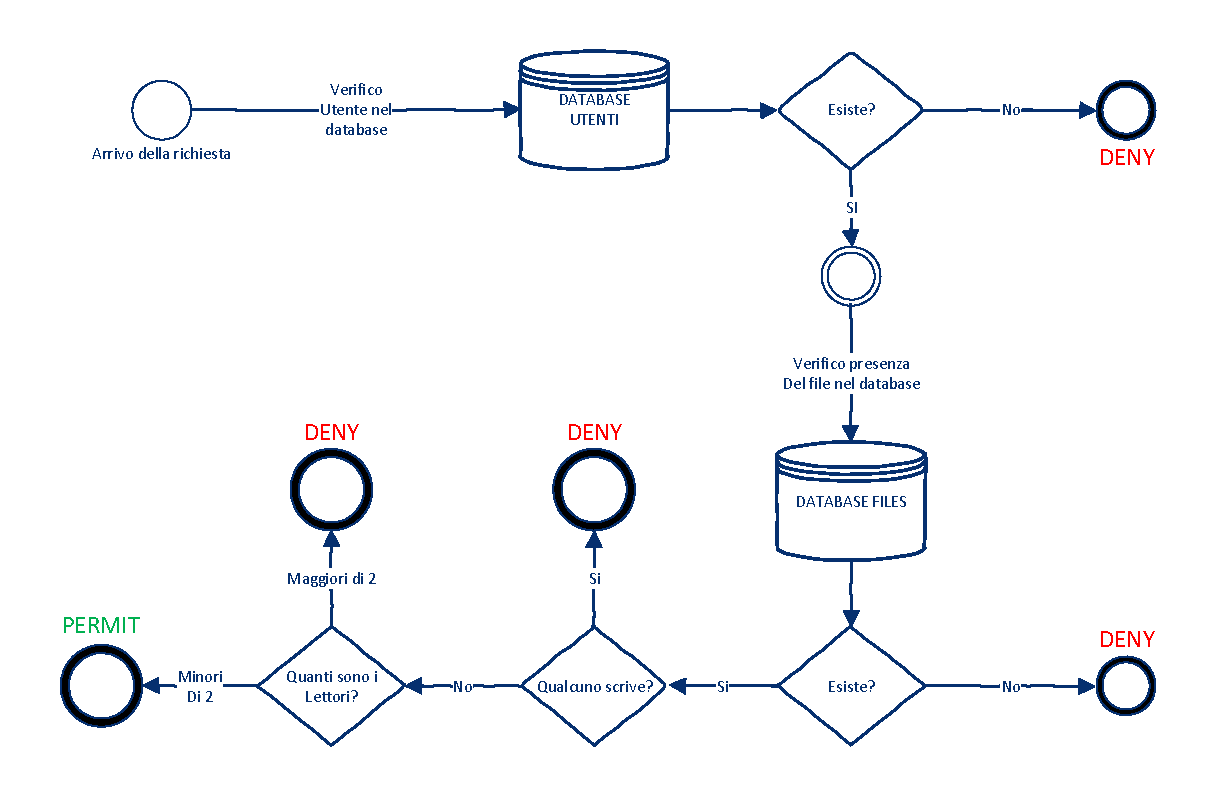
\includegraphics[width = 1.0\textwidth]{./Visio_Project/DiagrammaFlussoPrimoEsempio.pdf}
	%scale = 0.72, , trim=1.18cm 0 0 0
 	\caption{Diagramma di flusso del case study sull'accesso dei file}
 	\label{fig:diagrammaflussoprimoesempio}
\end{figure}

Se in un primo momento nessuno sta visualizzando o scrivendo un determinato file, ed un utente generico 
chiederà l'accesso in lettura per questo file, ovviamente il responso sarà positivo in quanto non viola la regola preposta prima.\par
Dopo un po' di tempo, mentre il primo sta ancora leggendo, un altro utente chiede l'accesso in scrittura, che gli viene negato.
In un istante di tempo successivo il primo utente sta continuando a leggere, ed anche il secondo utente vuole leggere. In questo caso viene dato responso positivo.\par
Infine, entrambi gli utenti smettono di leggere, ma uno di loro vuole apportare una modifica, allora richiede l'accesso in scrittura, che questa volta gli viene consentito poiché nessuno sta leggendo.



\subsection{Noleggio e acquisto di contenuti}
\label{sub:case2}

Un altro utilizzo possibile di \textit{Usage Control} riguarda l'analisi del comportamento passato. Un'azienda fornisce  ai propri clienti 
la possibilità di effettuare noleggi o acquisti di contenuti multimediali (musica, video, film, serie tv e via discorrendo).\par
In caso il contenuto fosse stato acquistato, l’acquirente potrà ottenere
l’accesso infinite volte per infinito tempo. Nel caso di noleggio invece
saranno presenti delle condizioni, come per esempio un numero massimo di visioni che quando superato non permette più di fruire del contenuto o una data di scadenza che, una volta oltrepassata,
impedirà l’ulteriore visione del file noleggiato in precedenza.\par
Come nell’esempio precedente viene mostrato un diagramma di flusso,
proposto Figura~\ref{fig:diagrammaflussosecondoesempio}, che permette di capire meglio il funzionamento questo sistema di \textit{Usage Control}. Innanzitutto viene verificata la presenza nei due relativi database dell'utente e del file richiesto, successivamente viene analizzata la richiesta, che può essere di tre tipi.
\begin{itemize}
\item Visione: nel caso la richiesta fosse di visione viene verificato se realmente l'utente ha diritto ad avere accesso a quella risorsa, e di conseguenza viene presa una decisione.
\item Acquisto: nel caso la richiesta fosse di acquisto verrà accreditato l'acquisto all'utente che ha effettuato la richiesta.
\item Noleggio: per questa forma ci sono due diverse tipologie, il noleggio a tempo e il noleggio a numero di visualizzazioni. Nel primo caso all'utente sarà concesso di vedere il file per un determinato periodo di tempo, mentre nel secondo il richiedente potrà visionare il file per un numero limitato di volte.
\end{itemize}
\begin{figure}[h]
 \centering 
	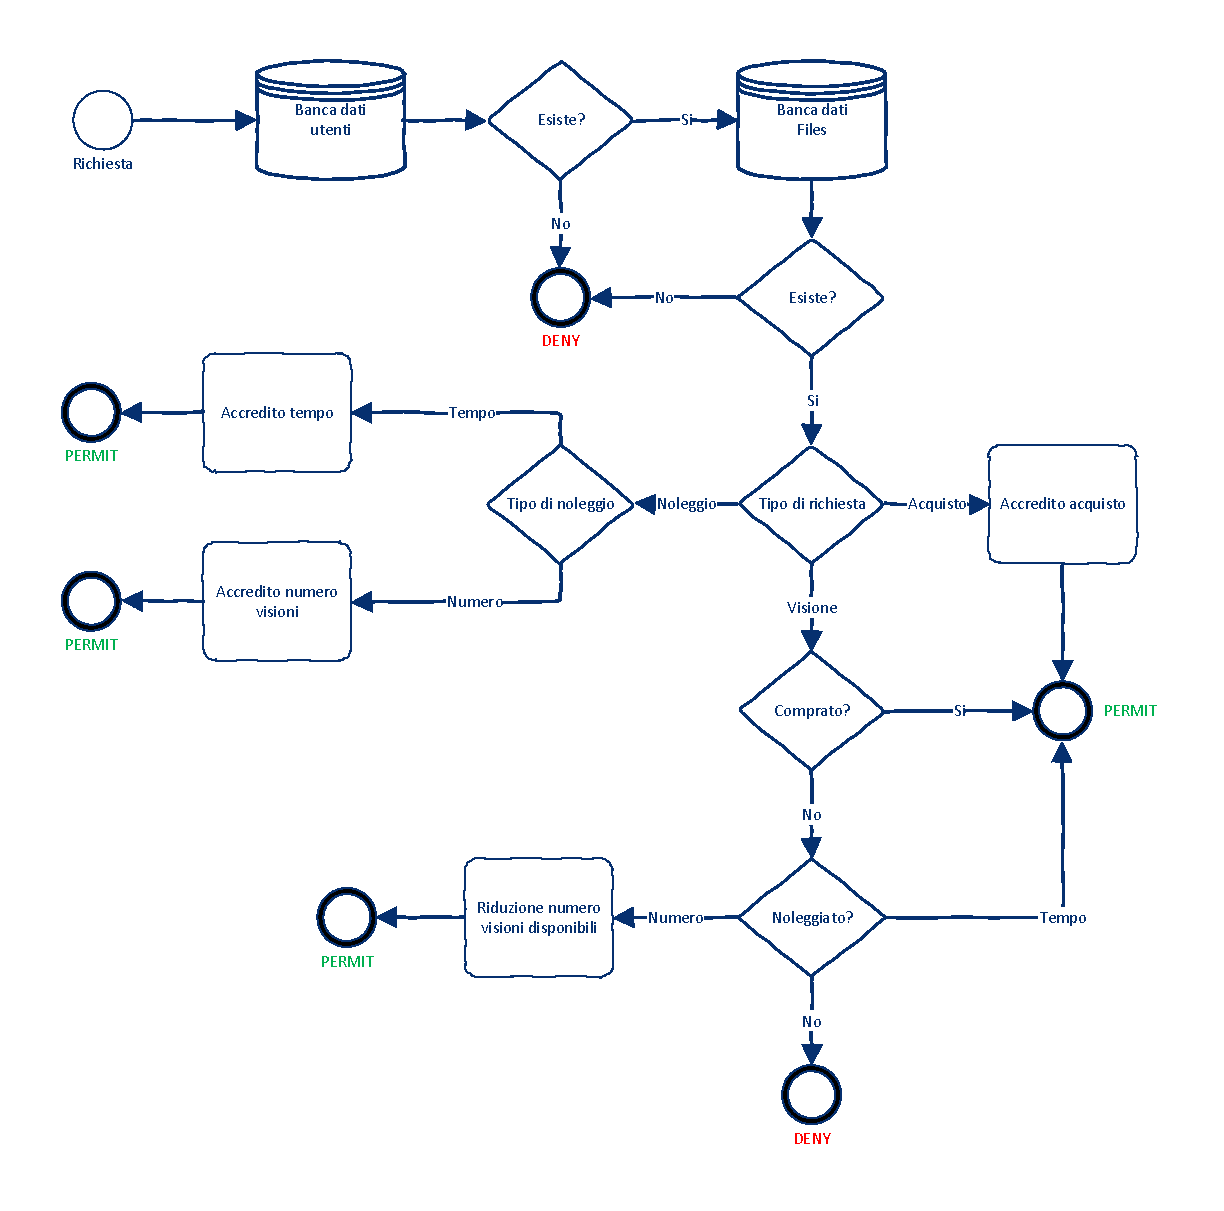
\includegraphics[width = 1.1\textwidth]{./Visio_Project/DiagrammaFlussoSecondoEsempio.pdf}
 \caption{Diagramma di flusso del case study sul noleggio e acquisto di contenuti}
 \label{fig:diagrammaflussosecondoesempio}
\end{figure}

\myChapter{Formal Access Control Policy Language}
\label{cap:facpl}
Negli anni molti linguaggi sono stati proposti per definire policy di access control. Uno di questi è stato rilasciato nel 2003 da parte di OASIS ed il suo nome è \textit{eXtensible Access Control Markup Language} (XACML). Questo linguaggio ha una sintassi basata su XML e fornisce caratteristiche avanzate per l'access control. Il problema fondamentale di XACML è che non ha una sintassi facile da leggere e da scrivere. \\
L'obiettivo di \textit{Formal Access Control Policy Language} (FACPL) è definire una sintassi alternativa per XACML in modo da renderlo più agevole da usare.
FACPL quindi è parzialmente inspirato a XACML, ma oltre ad introdurre una nuova sintassi ridefinisce alcuni aspetti aggiungendo nuove caratteristiche. Il suo scopo però non è sostituire XACML, ma fornire un linguaggio compatto ed espressivo per facilitare le tecniche di analisi attraverso tool specifici.

\section{Il processo di valutazione di FACPL}
\label{sec:valutazione_facpl}


\MyFigure{FACPL_EVALUATION.jpg}{Il processo di valutazione di FACPL}{1}
In figura \ref{fig:FACPL_EVALUATION.jpg} è mostrato il processo di valutazione delle policy definite in FACPL.
I componenti principali sono tre:
\begin{itemize}
\item{Policy Repository (PR)}
\item{Policy Decision Point (PDP)}
\item{Policy Enforcement Point (PEP)}
\end{itemize}
Le policy sono memorizzate nel PR, il quale le rende disponibili al PDP che deciderà, successivamente, se garantire l'accesso o meno (Primo step).
Nello step 2, quando il PEP riceve una richiesta, le credenziali di quest'ultima vengono codificate in una sequenza di attributi (ogni attributo è una coppia stringa valore) che, nello step 3, andranno a loro volta a formare una \textit{FACPL Request}.
Al quarto step il \textit{context handler} aggiungerà attributi di ambiente (per esempio l'ora di ricezione della richiesta) e manderà la richiesta al PDP.
A questo punto il PDP, tra il quinto e l'ottavo step, valuterà la richiesta e fornirà un risultato, il quale può eventualmente contenere delle \textit{obligations}.
La decisione del PDP può essere di quattro tipi, \textit{permit}, \textit{deny}, \textit{not-applicable} o \textit{indeterminate}.
Il significato delle prime due decisioni è facilmente intuibile, mentre per le ultime due vuol dire che c'è stato un errore durante la valutazione.
Gli errori possono essere di diverso tipo, e vengono gestiti attraverso algoritmi che combinano le decisioni delle varie policy per ottenere un risultato finale.
Le \textit{obligations} sono azioni, eseguite dal PEP, correlate al sistema di controllo degli accessi. Queste azioni possono essere di svariati tipi, come per esempio generare un file di log, o mandare una mail.
Allo step 13, sulla base del risultato delle \textit{obligations}, il PEP esegue un processo chiamato\textit{Enforcement} il quale restituirà un'altra decisione.
Quest'ultima decisione corrisponde alla decisione finale del sistema e può differire da quella del PDP.


\section{La sintassi di FACPL}
\label{sec:facpl_syntax}



\begin{table}[]
\footnotesize
\caption{Sintassi di FACPL}
\hrule
$
\begin{array}{@{\,}r@{\ \ }r@{\ }r@{\ \ }l@{\ }}
&&&\\[-.2cm]
{\textbf{Policy Authorisation Systems}} &
\mathit{PAS} & ::= & ( \,  \x{pep:} \, \mathit{EnfAlg}\ \ \x{pdp:}\, \mathit{PDP} \, )
\\[.2cm]
{\textbf{Enforcement algorithms}} &
\mathit{EnfAlg}
& ::= & \based \Sep \denyBiased \Sep \permitBiased 
\\[.2cm]
{\textbf{Policy Decision Points}} &
\mathit{PDP} & ::= & \pdpPol{\algNT\ }{\x{policies:} \, \mathit{Policy}^{+}}
\\[.2cm]
{\textbf{Combining algorithms}} &
\algNT & ::= & \permitOver \Sep \denyOver \Sep \denyUnless \Sep \permitUnless \\
&& \mid &
\firstApp \Sep \onlyOneApp \Sep \weakCon \Sep \strongCon 
\\[.2cm]
{\textbf{Policies}} &
\mathit{Policy} & ::= &
\ruleOpt{\mathit{Effect}\ \ \x{target:} \, Expr\ \ \x{obl:} \, \mathit{Obligation}^{*} \, } \\
&& \mid &
\{ \algNT\ \ \x{target:} \, Expr\ \ 
\x{policies:} \, \mathit{Policy}^{+} \ \ \x{obl:} \, \mathit{Obligation}^{*} \, \}
\\[.2cm]
{\textbf{Effects}} &
\mathit{Effect} & ::= & \permit \Sep \deny
\\[.2cm]
{\textbf{Obligations}} &
\mathit{Obligation} & ::= & [ \, \mathit{Effect} \ \ \mathit{ObType} \ \ \obl{Expr} \, ]
\\[.2cm]
{\textbf{Obligation Types}} &
\mathit{ObType} & ::= & M \Sep O
\\[.4cm]
\textbf{Expressions}&
\mathit{Expr} & ::= &
\mathit{Name} \Sep \mathit{Value}  \\
& & \mid &\x{and(\mathit{Expr}, \mathit{Expr})} \Sep \x{or(\mathit{Expr}, \mathit{Expr})} \Sep \x{not(\mathit{Expr})} \\
& & \mid &
 \x{equal(\mathit{Expr},\mathit{Expr})}  \Sep \x{in}(\mathit{Expr}, \mathit{Expr}) \\
& & \mid & \x{greater}\textrm{-}\x{than(\mathit{Expr},\mathit{Expr})} \Sep \x{add(\mathit{Expr} ,\mathit{Expr} )}\\ 
& & \mid & \x{subtract(\mathit{Expr} ,\mathit{Expr} )} \Sep \x{divide(\mathit{Expr} ,\mathit{Expr} )}\\
& & \mid & \x{multiply(\mathit{Expr} ,\mathit{Expr} )} \\[.2cm]
%
\textbf{Attribute Names} & 
\mathit{Name} & ::= & \mathit{Identifier}/\mathit{Identifier} \\[.2cm]
%
\textbf{Literal Values} &
\mathit{Value} & ::= & \x{true} \mid \x{false} \mid \mathit{Double} \mid \mathit{String} \mid \mathit{Date}
\\[.4cm]
{\textbf{Requests}} &
\mathit{Request} & ::= & {\attribute{\mathit{Name}}{\mathit{Value}}}^{+}
\\[.1cm]
\end{array}
$
\hrule
\label{tab:facpl_syntax}
\end{table}

\begin{table}[]
\footnotesize

\caption{Sintassi ausiliaria per le risposte}
\hrule
$
\begin{array}{@{\ }r@{\ \ \ \ }r@{\ }r@{\ \ }l@{\ }}

&&&\\[-.2cm]
{\textbf{PDP \ Responses }} &
\mathit{PDPResponse} & ::= & \langle \,\mathit{Decision} \ \ \ \mathit{FObligation}^* \rangle
\\[.2cm]
{\textbf{Decisions}} &
\mathit{Decision} & ::= & \permit \Sep \deny \Sep \notApp \Sep \indet
\\[.2cm]
{\textbf{Fulfilled obligations}} &
\mathit{FObligation} & ::= &  [ \, \mathit{ObType} \ \ \obl{\mathit{Value}} \, ]\\[.1cm]

\end{array}
$\\
\hrule
\label{tab:facpl_context_syntax}
\end{table}


La sintassi di FACPL è definita nella tabella \ref{tab:facpl_syntax}.
La sintassi è fornita come una grammatica di tipo EBNF, dove il simbolo ? corrisponde ad un elemento opzionale, il simbolo $*$ corrisponde ad una sequenza con un numero arbitrario di elementi (anche 0), ed il simbolo $+$ corrisponde ad una sequenza non vuota con un numero arbitrario di elementi.\\
Al livello più alto c'è il \textit{Policy Authorisation System (PAS)}, il quale definisce le specifiche del PEP e del PDP.
Il PEP è definito semplicemente come un \textit{enforcing algorithm} che sarà applicato per decidere quali decisioni verrà eseguito il processo di \textit{enforcement}. \\
Il PDP invece è definito come una sequenza (non vuota) di \textit{Policy}, ed un algoritmo di combining che combinerà i risultati di queste policy per ottenere un unico risultato finale.\\
Una \textit{policy} può essere una semplice \textit{rule} o una \textit{policy set}, quest'ultima avrà al suo interno altre \textit{policy set} o \textit{rule}, ed in questo modo viene formata una gerarchia di policy.\\
Un \textit{policy set} individua un target, che è una espressione che indica il set di richieste di accesso alla quale si applica la policy, una lista di \textit{obligations}, che definiscono azioni obbligatorie o opzionali che devono essere eseguite nel processo di \textit{enforcement}, una sequenza di altre \textit{policy}, ed un algoritmo per combinarle.\\
Una \textit{rule} includerà un \textit{effect}, che sarà permit o deny quando la regola è valutata correttamente, un target ed una lista di \textit{obligations}.\\
Le \textit{Expressions} sono formate da \textit{attribute names} e valori (per esempio boolean, double, strings, date).\\
Un \textit{Attribute Name} indica il valore di un attributo il quale può essere contenuto nella richiesta o nel contesto. FACPL usa per gli \textit{Attribute Name} una forma del tipo \textit{Identifier / Identifier }, dove il primo Identifier indica la categoria, ed il secondo il nome dell'attributo.
Per esempio \textit{Action / ID} rappresenta il valore di un attributo ID di categoria Action.\\
I \textit{Combining Algorithm} implementano diverse strategie che servono per risolvere conflitti tra le varie decisioni, restituendo alla fine un'unica decisione finale.\\
Una \textit{obligation} ha al suo interno un effect, un tipo, ed una azione eseguita dal PEP con la relativa \textit{Expression}.\\
Una \textit{request} consiste di una sequenza di attributi organizzati in categorie.\\
La risposta ad una valutazione di una richiesta FACPL è scritta usando la sintassi riportata in tabella \ref{tab:facpl_context_syntax}.
La valutazione in due step, descritta precedentemente in sezione~\ref{sec:valutazione_facpl}, produce due tipi di risultati. Il primo è la risposta del PDP, il secondo è una decisione, ovvero una risposta del PEP.
La decisione del PDP, nel caso in cui ritorni \texttt{permit} o \texttt{deny}, viene associata ad una lista, anche vuota, di fulfilled obligations.\\
Una \textit{fulfilled obligation} è una semplice coppia formata da un tipo (M o O) ed una azione i quali argomenti sono ottenuti dalla valutazione del PDP.

\section{La semantica di FACPL}
\label{sec:semantica_originale}

Molteplici sono le componenti di FACPL, e la semantica ora verrà informalmente analizzata.\cite{fullfacpl}
Prima verrà presentato il processo che porterà ad una risposta del PDP, successivamente il processo di enforcement del PEP.\\
Quando il PDP riceve una richiesta, per prima cosa valuta la richiesta sulle basi delle policy disponibili, successivamente determinerà un risultato combinando le decisioni ritornate da queste policy attraverso degli algoritmi di combining.\\
La valutazione della policy rispetto alla richiesta comincia verificando l'applicabilità alla richiesta, che è fatta valutando un espressione definita \textit{target}.\\
Si possono valutare due casi distinti:
\begin{itemize}
\item[-] Supponiamo che l'applicabilità dia esito positivo, nel caso ci sia una \textit{rule} sarà ritornato il valore risultato dalla valutazione di quest'ultima, mentre se c'è un \textit{policy set} il risultato è ottenuto valutando le policy contenute all'interno, e combinando i loro valori con un algoritmo specificato in fase di creazione del PDP. Successivamente a queste valutazioni verrà effettuato il fulfilment delle obligation contenute all'interno delle policy.
\item[-] Supponiamo ora che l'applicabilità non dia esito positivo, ovvero la valutaizone del \textit{target} restituisca \texttt{false}. In questo caso il risultato della policy sarà \texttt{not-app}. Mentre se \textit{target} restituisce un valore non booleano o ritorna un errore il risultato della policy sarà \texttt{indet}.
\end{itemize}
Valutare le espressioni corrisponde ad applicare degli operatori e risolvere i nomi degli attributi che contengono, e di conseguenza ricavarne un valore.\\
Se non è possibile trovare un attributo, magari perché non esiste, viene ritornato un valore speciale, chiamato \texttt{BOTTOM}. Questo valore può essere usato per implementare diverse strategie per gestire l'assenza di attributi. FACPL gestisce questo valore come una specie di \texttt{false}, quindi permette la mancanza di attributi senza la generazione di errori.\\
La valutazione di un espressione tiene conto anche dei tipi degli argomenti. Se l'argomento è del tipo aspettato l'operatore viene applicato correttamente, sennò, se un argomento è \texttt{BOTTOM} e nessun'altro è \texttt{error} viene ritornato \texttt{BOTTOM}, mentre se almeno uno di essi è \texttt{error}, viene ritornato \texttt{error}.\\
Con l'operatore \texttt{and} o \texttt{or} il trattamento sarà leggermente dievrso, in quanto \texttt{BOTTOM} viene ritornato solo se un argomento è tale e nessun'altro è \texttt{false} o \texttt{error}, mentre in caso contrario viene ritornato \texttt{error}.\\
La valutazione di una policy termina con il fulfillment di tutte le \texttt{obligations} le quali hanno il valore di applicabilità coincidente con quello ritornato dalla valutazione della policy. Quest'operazione consisten nel valutare tutte le espressioni presenti al interno delle \texttt{obligations} coinvolte nel processo. Se ci sarà un errore nel processo di fulfilment allora il risultato della policy sarà \texttt{indet}, altrimenti il risultato del fulfilment sarà uguale a quello della valutazione del PDP.\\
Gli algoritmi di combining, come detto prima hanno lo scopo di combinare le decisioni risultanti dalla valutazione delle richieste in accordo con le policy. Un'altra funzione che hanno è ritornare le \textit{obligations} corrette nel caso in cui la valutazione finale risulti \texttt{permit} o \texttt{deny}. Questa famiglia di algoritmi ha una strategia $\delta$ che viene usata per restituire le \textit{obligation}, e può essere di due tipi.
Il primo tipo è la strategia \texttt{all} (tutto), ovvero richiede la valtuazione di tutte le policy e ritorna le \texttt{fulfilled obligation} pertinenti a tutte le decisioni.\\
Il secondo tipo è la strategia \texttt{greedy} (golosa) prescrive che appena è ottenuta una decisione che non può cambiare a causa della valutazione di susseguenti policy nella sequenza di input, l'esecuzione si arresta.\\
Come ultimo step il risultato del PDP viene mandato al PEP per l'enforcement.
Il PEP per effettuare questo processo deve eseguire l'azione all'interno di ogni \texttt{fulfilled obligation} e decidere come comportarsi per le decisioni di tipo \texttt{not-app} e \texttt{indet.}\\
Per fare questo processo usa delle strategie. In particolare, l'algoritmo \texttt{deny-biased} (rispettivamente, \texttt{permit-based}) effettua l'enforcement dei \texttt{permit} (rispettivamente \texttt{deny}) solo quando tutte le corrispondenti obligations sono correttamente scaricate, mentre effettua l'enforcement dei \texttt{deny} (rispettivamente \texttt{permit}) in tutti gli altri casi. Invece, l'algoritmo di base lascia tutte le decisioni non cambiate ma, in caso di decisioni \texttt{permit} e \texttt{deny}, effettua l'enforcement di \texttt{indet} se un errore occorre quando si stanno rilasciando le \texttt{obligations}. Questo evidenzia che le \texttt{obligations} non solo influenzano il processo di autorizzazione, ma anche l'enforcement. Gli errori causati dalle \texttt{obligations} con tipo O vengono ignorati.


\myChapter{Implementare Usage Control in FACPL}

FACPL, fino alla versione descritta nel capitolo~\ref{cap:facpl}, non aveva la possibilità
di essere sfruttato per \textit{Usage Control}.\\
Grazie a delle nuove strutture implementate insieme al mio collega Filippo Mameli, adesso è possibile
usare FACPL per \textit{Usage Control}, introducendo miglioramenti descritti in~\ref{sec:usage_control}.\\
La nuova funzionalità consiste nel prendere decisioni tenendo conto delle richieste già effettuate.
Introdurre questa nuova estensione ha richiesto del lavoro sulla libreria, in quanto è stato necessario aggiungere
nuove componenti e di conseguenza modificare il processo di valutazione di una policy.
Infine è stato necessario anche introdurre delle modifiche alla sintassi del linguaggio in modo da poterle sfruttare 
facilmente.

\section{Estensione del processo di Valutazione} % (fold)
\label{sec:estensione_del_processo_di_valutazione}
Il processo di valutazione è stato esteso per via delle modifiche introdotte. 
Rispetto al processo di valutazione standard, descritto in sezione~\ref{sec:valutazione_facpl}, sono state aggiunte
componenti al grafico, rendendolo così adatto allo \textit{Usage Control}, in particolare alla valutazione di 
richieste basate sul comportamento passato.
\MyFigure{evalStatus}{Nuovo processo di valutazione in FACPL}{1}
Come si nota in figura \ref{img:evalStatus} è stato aggiunto un componente alla struttura della valutazione.
Questo componente è lo \status \ (Stato), ovvero un semplice contenitore di un nuovo tipo di attributi.
I nuovi attributi vengono chiamati \statusattribute. Ovviamente quest'estensione non modifica il comportamento nel caso di assenza di stato, di conseguenza la valutazione rimane inalterata rispetto a quella descrita precedentemente, mentre viene modificata nel caso in cui lo stato sia presente in modo da gestire correttamente la presenza di esso.\\
Analizziamo quindi, a scopo esemplificativo, il secondo caso, ovvero quando lo stato è presente. Inizialmente viene definito il sistema, che ora ha quattro componenti principali:
\begin{itemize}
	\item[-]{Policy Repository (PR)}
	\item[-]{Policy Decision Point (PDP)}
	\item[-]{Policy Enforcement Point (PEP)}
	\item[-]{Status}
\end{itemize}
Fino al quarto step il comportamento è analogo a quello precedente, mentre cambia negli step successivi.\\
Al quinto step il \textit{PDP} non necessiterà solo dei normali attributi d'ambiente, ma necessiterà anche degli \statusattribute \ coinvolti nella richiesta effettuata. Il \textit{Context Handler} quindi non andrà solo a fare la ricerca all'interno dell'environment, ma andrà a cercare anche gli \statusattribute \ all'interno dello \status.\\
A questo punto, quando il PDP avrà tutte le informazioni necessarie si potrà passare alla vera e propria valutazione della richiesta che avviene come sempre.\\
Nel caso in cui viene restituto \texttt{Permit} o \texttt{Deny} è necessario fare l'enforcement della risposta del PDP. Questo processo differisce dal precedente poiché ora sono state implementate nuove azioni sullo stato che devono essere eseguite. Una volta effettuato l'enforcement viene restituta la decisione finale.\\
Prendendo il primo esempio citato in sezione \ref{sec:usage_control} la valutazione procederebbe in questo modo. Bob richiederà la lettura di un determinato file. Quindi la richiesta conterrà tre attributi, uno che indica il nome dell'utente che effettua la richiesta, il secondo che contiene il nome del file a cui si effettuerà l'accesso, e il terzo che conterrà il nome dell'azione da effettuare. La policy invece sarà strutturata come \textit{"Se il nome è Bob, il file è corretto e nessuno sta scrivendo o ci sono meno di due utenti che leggono, allora permetti, altrimenti nega" }.\\
Il PDP però ha bisogno di più attributi per valutare la richiesta, in quanto necessita anche di attributi esterni alla policy che riguardano il numero di utenti che stanno accedendo al file richiesto, questi attributi sono gli \statusattribute. Per la loro gestione sarà necessario utilizzare la funzionalità che riguarda l'Usage Control, il PDP richiederà al \textit{Context Handler} questi attributi, il quale andrà cercarli nello \status. Quest'ultimo li fornirà e verranno direttamente mandati al PDP per la valutazione della richiesta.\\
Se la richiesta avrà esito positivo, allora vuol dire che Bob avrà accesso al file, e quindi lo stato andrà aggiornato. La risposta del PDP a questo punto andrà al PEP per l'enforcement il quale avrà il compito di aggiornare lo stato. Sostanzialmente lo stato viene aggiornato semplicemente incrementando l'attributo riguardante il numero di lettori di un'unità.



% section estensione_del_processo_di_valutazione (end)

\section{Estensione Linguistica} % (fold)
\label{sec:estensione_linguistica}
Per implementare queste nuove funzionalità è stata modificata anche la grammatica di FACPL.
Nella grammatica estesa sono state aggiunte nuove regole di produzione e simboli terminali che 
codificano le nuove funzionalità.\\

\begin{table}[h]
\centering
\small
\caption{Sintassi di $FACPL_{PB}$} 
$
\begin{array}{@{\,}r@{\ \ }r@{\ }r@{\ \ }l@{\ }}

&&&\\[-.2cm]
{\textbf{Policy Authorisation Systems}} &
\mathit{PAS} & ::= & ( \,  \x{pep:} \, \mathit{EnfAlg}\ \ \x{pdp:}\, \mathit{PDP} \, \  \x({status:}\, \mathit{
[Attribute]^+})^*)
\\[.2cm]
{\textbf{Attribute}} &
\mathit{Attribute}
& ::= & (\mathit{Type} \ \mathit{Identifier} \ (= Value )^{?})
\\[.2cm]
{\textbf{Type}} &
\mathit{Type}
& ::= & \x{int} \ | \ \x{boolean} \ | \ \x{date} \ | \ \x{float}
\\[.2cm]
{\textbf{Enforcement algorithms}} &
\mathit{EnfAlg}
& ::= & \based \Sep \denyBiased \Sep \permitBiased 
\\[.2cm]
{\textbf{Policy Decision Points}} &
\mathit{PDP} & ::= & \pdpPol{\algNT\ }{\x{policies:} \, \mathit{Policy}^{+}}
\\[.2cm]
{\textbf{Combining algorithms}} &
\algNT & ::= & \permitOver \Sep \denyOver \Sep \denyUnless \Sep \permitUnless \\
&& \mid &
\firstApp \Sep \onlyOneApp \Sep \weakCon \Sep \strongCon 
\\[.2cm]
\textbf{fulfilment strategies} & \delta
& ::= & 
\greedy \Sep \all 
\\[.2cm]
{\textbf{Policies}} &
\mathit{Policy} & ::= &
\ruleOpt{\mathit{Effect}\ \ \x{target:} \, Expr\ \ \x{obl:} \, \mathit{Obligation}^{*} \, } \\
&& \mid &
\{ \algNT\ \ \x{target:} \, Expr\ \ \\
&&  &
\x{policies:} \, \mathit{Policy}^{+}  \ \ \x{obl:} \, \mathit{Obligation}^{*} \, \}
\\[.2cm]
{\textbf{Effects}} &
\mathit{Effect} & ::= & \permit \Sep \deny
\\[.2cm]
{\textbf{Obligations}} &
\mathit{Obligation} & ::= & [ \, \mathit{Effect} \ \ \mathit{ObType} \ \ \obl{Expr} \, ]
\\[.2cm]
{\textbf{PepAction}} & \mathit{PepAction} & ::= & \, \x{add(\mathit{Attribute}, int)} \Sep \x{flag(\mathit{Attribute}, boolean)} \\ 
&& & \Sep \x{sumDate(\mathit{Attribute}, date)} \Sep \x{div(\mathit{Attribute}, int)} \\
&& & \Sep \x{add(\mathit{Attribute}, float)} \ \Sep \x{mul(\mathit{Attribute}, float)} \\
&& & \Sep \x{mul(\mathit{Attribute}, int)} \ \Sep \x{div(\mathit{Attribute}, float)} \\
&& & \Sep \x{sub(\mathit{Attribute}, int)} \ \Sep \x{sub(\mathit{Attribute}, float)} \\
&& & \Sep \x{sumString(\mathit{Attribute}, string)} \\ 
&& & \Sep \x{setValue(\mathit{Attribute}, string)}\\
&& & \Sep \x{setDate(\mathit{Attribute}, date)}  
\\[.2cm]
{\textbf{Obligation Types}} &
\mathit{ObType} & ::= & M \Sep O
\\[.4cm]
\textbf{Expressions}&
\mathit{Expr} & ::= &
\mathit{Name} \Sep \mathit{Value}  \\
& & \mid &\x{and(\mathit{Expr}, \mathit{Expr})} \Sep \x{or(\mathit{Expr}, \mathit{Expr})} \Sep \x{not(\mathit{Expr})} \\
& & \mid &
 \x{equal(\mathit{Expr},\mathit{Expr})}  \Sep \x{in}(\mathit{Expr}, \mathit{Expr}) \\
& & \mid & \x{greater}\textrm{-}\x{than(\mathit{Expr},\mathit{Expr})} \Sep \x{add(\mathit{Expr} ,\mathit{Expr} )}\\ 
& & \mid & \x{subtract(\mathit{Expr} ,\mathit{Expr} )} \Sep \x{divide(\mathit{Expr} ,\mathit{Expr} )}\\
& & \mid & \x{multiply(\mathit{Expr} ,\mathit{Expr} )}  \Sep \x{less}\textrm{-}\x{than(\mathit{Expr}, \mathit{Expr})}\\
\\[.2cm]
%
\textbf{Attribute Names} & 
\mathit{Name} & ::= & \mathit{Identifier}/\mathit{Identifier} \ | \ \mathit{Status}/\mathit{Identifier}\\[.2cm]
%
\textbf{Literal Values} &
\mathit{Value} & ::= & \x{true} \mid \x{false} \mid \mathit{Double} \mid \mathit{String} \mid \mathit{Date}
\\[.4cm]
{\textbf{Requests}} &
\mathit{Request} & ::= & {\attribute{\mathit{Name}}{\mathit{Value}}}^{+}
\\[.1cm]
\end{array}
$
\label{tab:facpl_new_syntax}
\end{table}




Come è facilmente osservabile dalla consultazione della tabella~\ref{tab:facpl_new_syntax} le aggiunte rispetto alla tabella riporta in sezione~\ref{sec:facpl_syntax} sono state diverse, vediamo adesso quali sono.\\
La prima modifica che risulta evidente è nel PAS, ovvero nella definizione del sistema. L'aggiunta è stata lo \status, ovvero un contenitore di attributi.
Uno \status \ è della forma $$(status: Attribute^+)^?$$ questo significa che se lo \status \ è presente sarà formato da uno o più \textit{Attribute}.\\
Passiamo ora a descrivere \textit{Attribute} che è della forma $$(Type\ Identifier (= Value)^?)$$
questo tipo particolare di attribute, che è lo \statusattribute \ descritto in precedenza, è formato innanzitutto da un \textit{Type}, dopo il tipo è richiesta una generica stringa chiamata \textit{Identifier}, che sarà un generico nome da dare all'attributo, infine viene richiesto un \textit{Value}, ovvero un valore, che in questo caso è opzionale, all'atto pratico vuol dire che l'attributo di stato potrà essere inizializzato con un valore oppure potrà essere solamente definito, lasciando che il valore sia quello di default.\\
\textit{Type} è il tipo che avrà l'attributo di stato, e potrà essere \texttt{int, boolean, date o float}.\\
La regola \textit{PepAction} è stata modificata in modo tale che includesse nuove funzioni per operare matematicamente sugli attributi di stato.
Queste nuove funzioni sono:
\begin{itemize}
	\item \textit{add(Attribute, \texttt{int})}
	\item \textit{add(Attribute, \texttt{float})}
	\item \textit{div(Attribute, \texttt{int})}
	\item \textit{div(Attribute, \texttt{float})}
	\item \textit{sub(Attribute, \texttt{int})}
	\item \textit{sub(Attribute, \texttt{float})}
	\item \textit{mul(Attribute, \texttt{int})}
	\item \textit{mul(Attribute, \texttt{float})}
	\item \textit{flag(Attribute, \texttt{boolean})}
	\item \textit{sumDate(Attribute, \texttt{date})} 
	 
\end{itemize}
Infine l'ultima regola di produzione modificata è stata quella riguardante \textit{Attribute Names}, in questo caso è stata semplicemente aggiunto, a fianco di \textit{Identifier/Identifier}, una nuova produzione \textit{Status/Identifier}. Questa nuova produzione serve semplicemente per permettere il confronto tra attributi di stato attraverso le già esistenti \textit{Expression}.
La sintassi delle risposte è rimasta invariata.
Vediamo ora un esempio di questa nuova sintassi, prenderemo spunto da un caso già trattato in precedenza nella sezione~\ref{sec:estensione_del_processo_di_valutazione}.
%SOSTITUIRE CON LISTINGS PER FACPL
\lstinputlisting[language = FACPL, caption = {Esempio per la sintassi}\label{lst:esempio_sintassi}]{./Source/first_example_facpl}
In questo esempio (Codice \ref{lst:esempio_sintassi}) si può vedere come nel PAS è stato definito uno stato, con al suo interno uno solo attributo inizializzato con valore 0.
Successivamente si può notare nella \textit{Rule} che viene fatto un controllo sul valore di quest'attributo.
Infine nella \textit{Obligation} si può notare come viene aggiornato lo stato dell'attributo in base al risultato della valutazione della \textit{Rule}.
% section estensione_linguistica (end)

\section{Semantica} % (fold)
\label{sec:semantica}

% section semantica (end)


\section{Esempi} % (fold)
\label{sec:esempi}

% section esempi (end)


\section{Estensione della libreria FACPL} % (fold)
\label{sec:estensione_della_libreria_facpl}

% section estensione_della_libreria_facpl (end)
\myChapter{Estensione della libreria FACPL}
\label{cap:estensione_libreria}
Il linguaggio \ac{FACPL} è supportato da una libreria Java. Per supportare l'estensione proposta
abbiamo esteso questa libreria. Per ovvi motivi verranno mostrate solo alcune parti delle modifiche effettuate, ma 
il codice completo si può comunque trovare su GitHub all'url \url{https://github.com/andreamargheri/FACPL}.\par
In Sezione~\ref{sec:imp_stato} è presentata l'implementazione in Java dello stato e degli attributi di stato. Lo stato ha richiesto anche l'implementazione di altre componenti come le funzioni per modificare gli attributi e l'estensione del \ac{PEP}.
Nella Sezione~\ref{sec:estensione_politiche} è trattata l'estensione delle politiche. In particolare si parla di come è stato possibile 
effettuare comparazioni su attributi di stato e di come sono state estese le obligation.
In Sezione~\ref{sec:plugin_eclipse} viene mostrato come è stato esteso il plugin di \ac{FACPL} per supportare le nuove estensioni.
Infine, in Sezione~\ref{sec:implementazione_esempi}, vengono presentati in Java i case study già proposti in \ref{sec:casi_studio} e
\ref{sec:esempi}
\section{Implementazione Stato}
\label{sec:imp_stato}
Il primo passo per estendere la libreria è stato la creazione di uno \status, che è modellato da una semplice classe 
di cui ne verrà mostrato un pezzo in Codice~\ref{lst:PezzoStatus1}. Il fulcro di questa classe è una Hashmap con key parametrizzata a 
\statusattribute \ e valore corrispondente parametrizzato ad Object. Questa Hashmap associa quindi ad uno \statusattribute\ il suo valore corrispondente.
\myIjava{status.java}{Stralcio della classe Status}{1}{7}{PezzoStatus1}

In Figura~\ref{fig:statusUML.png} è possibile vedere la relazione che intecorre tra lo stato ed i suoi attributi. 
\MyFig{statusUML.png}{Grafico UML delle classi Status e StatusAttribute}{1}{H}
Come si vede dal grafico UML in Figura \ref{fig:statusUML.png} la classe che modella lo stato include altri due metodi non mostrati in Codice~\ref{lst:PezzoStatus1}. Per via dei rispettivi nomi i metodi risultano abbastanza autoesplicativi, per questo ne verrà mostrato solo uno in Codice~\ref{lst:PezzoStatus2}.
\myIjava{status.java}{Set Attribute della classe Status}{32}{37}{PezzoStatus2}

\subsection{Status Attribute}
\label{sub:status_attribute}
Uno Status Attribute è un tipo particolare di attributo. Come si può vedere dalla Figura \ref{fig:statusUML.png} per creare questo nuovo tipo è stata estesa una classe già esistente, ovvero quella che rappresenta gli attributi normali.
\myIjava{SA.java}{Classe Status Attribute}{1}{6}{StatusAttribute}
Nel Codice \ref{lst:StatusAttribute} è possibile vedere il costruttore e i campi di questa nuova classe. In aggiunta agli attributi normali è stato aggiunto un Tipo, che può essere:
\begin{itemize}
	\item Int
	\item String
	\item Date
	\item Boolean
	\item Double
\end{itemize}
Il costruttore riceve due parametri: l'ID e il tipo. In questo metodo viene invocato il costruttore della superclasse dove gli viene passata una categoria fissata, ovvero \textit{Status} e l'ID.
\subsection{Funzioni su Status Attribute}
\label{sub:funzioni_status_attribute}
Le funzioni sugli status attribute sono operazioni che ne vanno a modificare il valore. Derivano tutte da un unica interfaccia mostrata in Codice~\ref{lst:IExpressionFunctionStatus.java}, che avrà come unico metodo quello che eseguirà la vera e propria operazione.
\myjava{IExpressionFunctionStatus.java}{Interfaccia per le operazioni}
Dal grafico UML in Figura~\ref{fig:functionarith.png} si vede chiaramente che ci sono due grandi gerarchie di classi: quelle che fanno operazioni sui numeri e quelle che fanno operazioni sulle stringhe.
Per eseguire un'operazione è sufficiente istanziare una classe che estende \textit{StringOperationStatus} o \textit{MathOperationStatus}, e chiamare l'unico metodo definito nell'interfaccia in Codice \ref{lst:IExpressionFunctionStatus.java} passandogli i parametri corretti. La sottoclasse istanziata eredita il metodo \textit{evaluateFunction} dalla superclasse ed implementa il metodo astratto \textit{op}. Il metodo \textit{evaluateFunction} implementato nella superclasse, in base ai parametri che gli vengono passati, si fa restituire da una factory, in base al tipo del attributo, il valutatore corretto che passerà a sua volta al metodo astratto \textit{op}. Il valutatore è una classe dove è scritto il codice Java che eseguirà l'operazione vera e propria.
Nel Codice~\ref{lst:addStatus.java} viene mostrata la sottoclasse che si occupa della somma su numeri. Si nota subito che questa è una sottoclasse di \textit{MathOperationStatus} e che implementa solo il metodo \textit{op}.
\myjava{addStatus.java}{Add Status}
La ragione dietro la verbosità creata dall'utilizzo di un valutatore, oltre che da una moltitudine di classi e sottoclassi, potrebbe sembrare superflua; ciononostante quest'ultima è una scelta lungimirante, in quanto in futuro sarà più agevole implementare nuovi tipi di attributo e relative funzioni su di essi.

\begin{sidewaysfigure}
	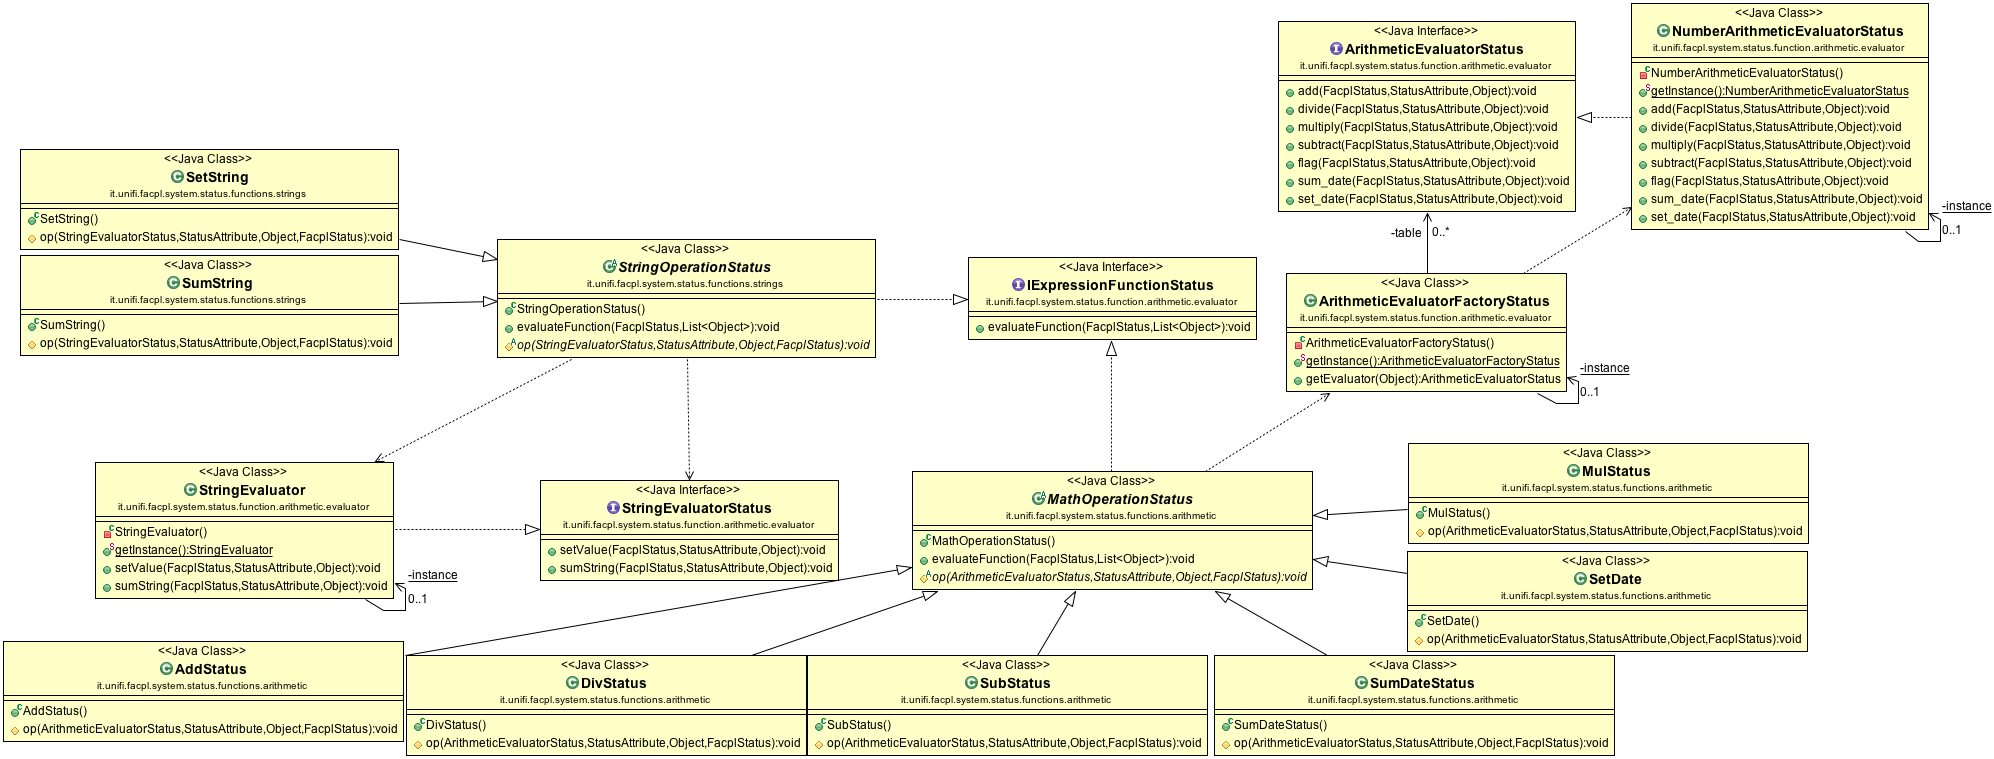
\includegraphics[width=1.03\linewidth, trim = 10cm 0 0 0]{functionarith2.png}
    \caption{Grafico UML per la gerarchia di funzioni aritmetiche}
    \label{fig:functionarith.png}
\end{sidewaysfigure}

\subsection{Estensione del PEP}
\label{sub:estensione_PEP}
La struttura del \ac{PEP} è rimasta pressoché uguale in quanto non è stato esteso, bensì modificato.
In seguito alla valutazione di una policy il \ac{PDP} darà una risposta, su questa risposta il \ac{PEP} dovrà effettuare il suo processo di enforcement.
Durante questo processo vengono valutate le \textit{Obligation} in modo che l'operazione al loro interno sia eseguita; il metodo che effettua questo compito è 
\textit{dischargeObligation}. La modifica ha coinvolto proprio quest'ultimo, in quanto è bastato aggiungere un \textit{else if}, mostrato in Codice~\ref{lst:PEP}, a quelli già presenti.
\myIjava{PEP.java}{Discharge delle Fulfilled Obligation di stato}{102}{106}{PEP}
In questo modo vengono prese in considerazione anche le nuove Obligation Status, quindi ora il \ac{PEP}, durante il suo processo di enforcement, riuscendo ad eseguire questo nuovo tipo di Obligation potrà modificare lo stato.


\section{Estensione delle politiche}
\label{sec:estensione_politiche}

Le politiche, in seguito all'estensione, vengono valutate basandosi anche sullo stato indi per cui si è reso necessario estendere il contesto intorno a cui sono valutate. Come mostrato in Figura~\ref{fig:contextrequest.png} l'estensione del contesto si ottiene mediante la creazione di una nuova classe, a estensione di quella esistente.
\MyFig{contextrequest.png}{Contesto}{0.40}{H}
La nuova classe ContextRequest\_Status contiene lo stato sotto forma di campo privato. L'accesso allo stato è effettuato tramite il metodo getContextRequestValue (Codice~\ref{lst:cxtReq}), che in questa sottoclasse è stato riscritto.
\myIjava{context_request_status.java}{Discharge delle Fulfilled Obligation di stato}{37}{55}{cxtReq}
Questo metodo riceve come parametro un attributo, ed in base al suo tipo andrà a cercarlo nello stato o nell'ambiente.

\subsection{Funzioni di controllo su status}
\label{sub:funzioni_controllo_status}

Il \ac{PDP} per poter valutare correttamente le richieste deve avere la possibilità di comparare anche questo nuovo tipo di attributi.
Raggiungere quest'obiettivo non è stato difficile in quanto la struttura era già esistente e funzionante, ed essendo i nuovi attributi soltanto un estensione di quelli 
creati in precedenza è stato possibile usarla senza alcun tipo di problema.\par

\MyFig{comparisonUML.png}{Comparatori}{1.07}{H}

Come nel caso delle funzioni di modifica dello stato, la struttura è basata su un factory che ritorna il valutatore corretto in base al tipo su cui deve essere effettuato il confronto.

\subsection{Obligation}
\label{sub:estensione_obligation}
Le \textit{Obligation} sono state estese introducendo un nuovo tipo chiamato \textit{Obligation Status}, questo tipo particolare di \textit{Obligation} serve per andare ad eseguire azioni sullo stato.
Nella libreria sono presenti due tipi fondamentali di \textit{Obligation}, i primi sono quelli a livello sintattico, i secondi, chiamati \textit{FulfilledObligations} sono quelli pronti ad essere valutati. Vediamo adesso come sono state estesi quelle a livello sintattico. \par
Per eseguire questa estensione è stato reso necessario un refactoring, per prima cosa è stato astratto tutto il comportamento comune in una superclasse astratta, successivamente è stata creata la nuova classe che modella questo nuovo tipo.
Il refactoring ha coinvolto anche il metodo che si occupa del \textit{Fulfilling} delle \textit{Obligation} in quanto ora deve creare anche questo nuovo tipo, la scelta più ovvia è stata creare un metodo astratto implementato nelle due sottoclassi che viene chiamato dalla superclasse per creare il tipo corretto.
\myIjava{absObl.java}{Parte rifattorizzata del metodo che si occupa del fulfilling}{16}{18}{fulfilabs}
\myIjava{oblStat.java}{CreateObligation nelle status}{17}{24}{createoblstat}
\myIjava{oblNorm.java}{CreateObligation nelle normali}{11}{14}{createoblnorm}
La \textit{Obligation} di stato necessiterà anche di argomenti su cui eseguire l'azione, che le verranno passati in fase di costruzione. \par
Alla fine della valutazione il \ac{PDP} crea un oggetto di tipo \textit{AuthorisationPDP} che conterrà la decisione e una lista di \textit{FulfilledObligation}, quest'ultime poi andranno al \ac{PEP} per la loro valutazione. Vediamo ora come sono state implementate. \par
Anche in questo caso è stato necessario un refactoring analogo a quello fatto per le prime.
\myIjava{FulOblStat.java}{Peculiarità della classe FulfilledObligationStatus}{1}{15}{pecfulstat}
Come si può notare, in fase di costruzione gli verrà passato un oggetto di tipo \textit{IExpressionFunctionStatus} che sarà l'azione che andrà a eseguire sullo stato. Quest'azione andrà realmente ad essere eseguita quando verrà chiamato dal \ac{PEP} il metodo \textit{evaluateObl}. \par
Il \ac{PEP} nella fase di enforcement effettua la valutazione delle \textit{Obligation}, in questo caso le modifiche per permettere al sistema di eseguirle sono state minime: è bastato modificare il metodo \textit{DischargeObligation} in modo che quando gli viene passata una \textit{AbstractFulfilledObligation} chiamasse il metodo \textit{evaluateObl} .
\myIjava{PEP.java}{Discharge delle Fulfilled Obligation di stato}{102}{106}{PEP}
\begin{sidewaysfigure}[H]
    \centering
	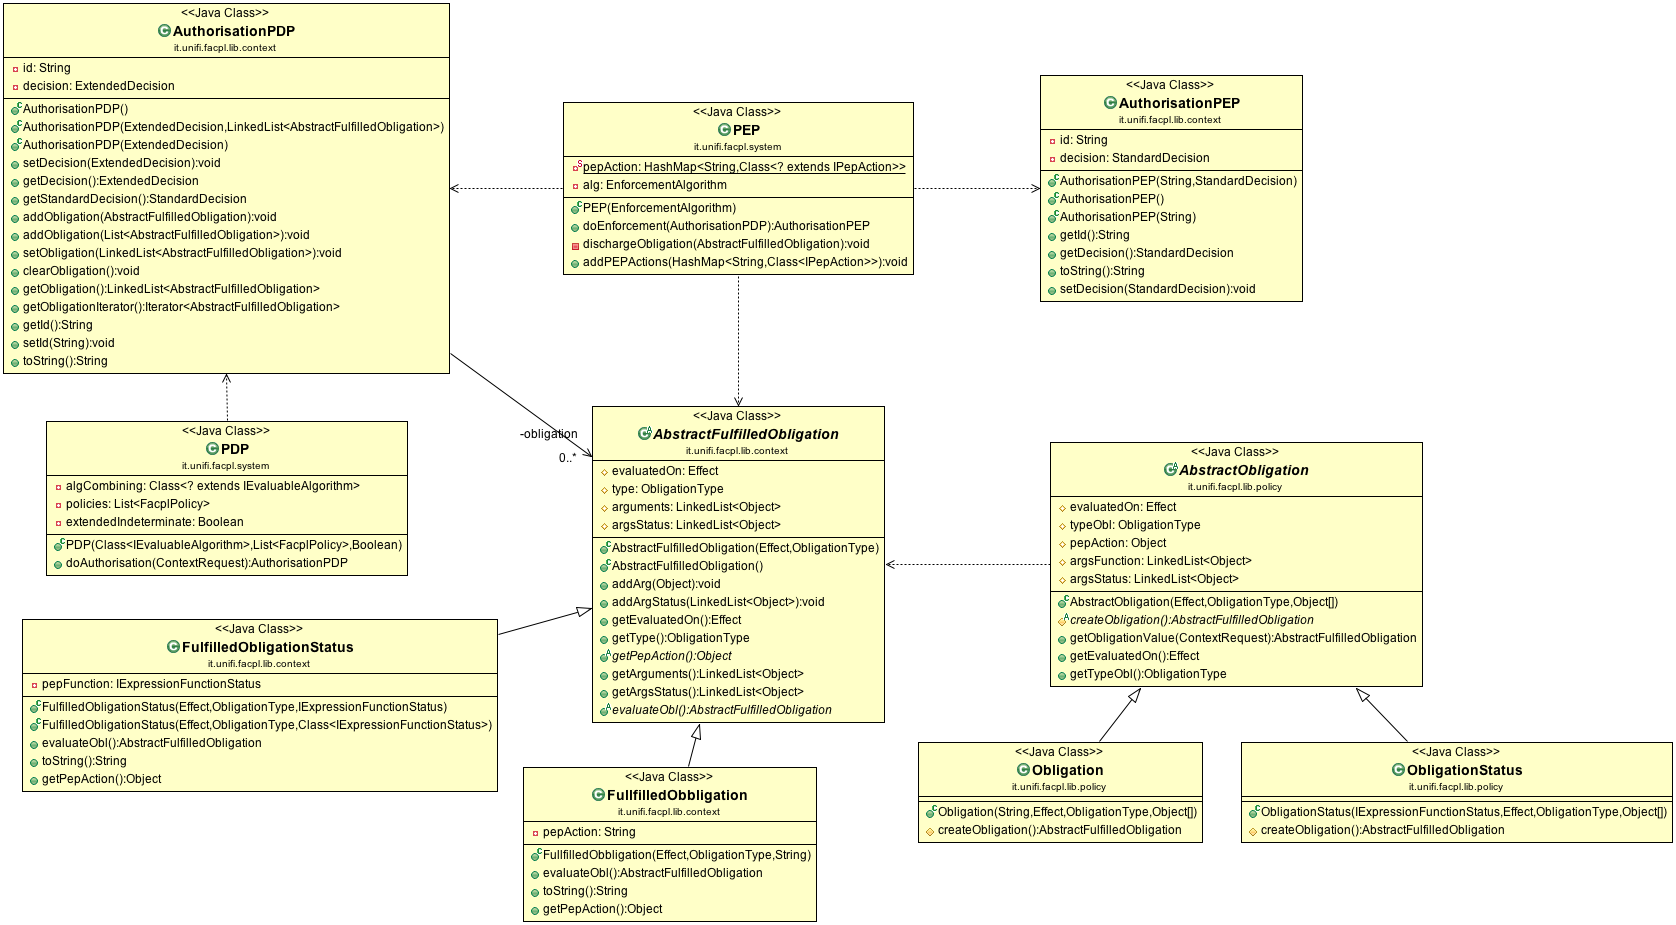
\includegraphics[width=1.1\linewidth]{obl.png}
    \caption{Relazioni tra Obligation e PEP}
    \label{fig:obl.png}
\end{sidewaysfigure}




\section{Plugin Eclipse}
\label{sec:plugin_eclipse}

La sintassi di \ac{FACPL} è definita in Xtext. Quest ultimo è un framework, basato su Java, per lo sviluppo di linguaggi, e fa uso di Xtend per tradurre da \ac{FACPL} a codice Java.
XTend ha le sue radici in Java, ma si concentra maggiormente su aspetti come una sintassi più concisa ed altre funzionalità come l'inferenza sui tipi, l'overload degli operatori o l'estensione dei metodi. 
È principalmente un linguaggio Object-oriented, ma integra caratteristiche tipiche di un linguaggio funzionale, come ad esempio le Lambda Expression. Il sistema dei tipi di XTend è lo stesso di Java, ed è quindi statico.\par
Inizialmente è stata estesa la grammatica, introducendo i nuovi costrutti come lo Stato, gli \statusattribute \ e le nuove Obligation.
Successivamente sono state scritte le regole di traduzione in Xtend in modo che il codice scritto in $FACPL_{PB}$ venisse tradotto in Java.\par
Il primo passo è stato quello di creare gli attributi e lo stato per poi integrarli nel PAS.
Sono state scritte tre nuove regole di produzione mostrate in Figura~\ref{fig:reg_prod}
\MyFig{reg_prod}{Regole di produzione per lo stato}{1}{H}
La prima regola serve ad introdurre lo stato all'interno del PAS.
La seconda definisce lo stato come un insieme di attributi dichiarabili.
Nella terza regola sono definiti gli attributi, i quali avranno un tipo, un nome ed un valore.
La quarta regola invece sono gli attributi dichiarabili, ovvero degli attributi racchiusi tra parentesi tonde.\par
Lo step successivo è stato estendere le Obligation e le espressioni.
Per estendere le obligation è stato necessario modificare la regola ed introdurre nuove funzioni. Per introdurre la valutazione degli \statusattribute \ è stata estesa la regola Function. Tutte queste modifiche sono mostrate in Figura~\ref{fig:obl_fun}.
\MyFig{obl_fun}{Regole di produzione per obligation e le espressioni}{1}{H}
Dopo aver esteso la grammatica sono state estese anche le regole di traduzione. Mostriamo ora com'è stato realizzato lo stato.
Chiamando la funzione in Figura~\ref{fig:stato_xtend} verrà generata una sequenza di caratteri che verrà successivamente scritta su un file Java, creando così la classe che andrà a definire lo stato.
\MyFig{stato_xtend}{Stato in Xtend}{1.2}{H}
Lo stato è formato da una hashmap contentente una serie di attributi. Ovviamente quest'ultimi saranno l'unica parte variabile di questa classe, quindi per far sì che vengano ogni volta aggiunti in modo corretto è presente un ciclo che scorre i vari attributi e per ognuno di essi genera il codice Java necessario per istanziarli. \par
Il plugin si presenta come in Figura~\ref{fig:plugin}. Le funzionalità di questo plugin sono proprie di un ambiente di sviluppo, in quanto offre l'autocompletamento e il syntax highlighting. 
\MyFig{plugin}{Plugin di \ac{FACPL}}{0.75}{H}



\section{Esempi}
\label{sec:implementazione_esempi}

In questa sezione vengono ripresi i casi di studio già dicussi in Sezione \ref{sec:esempi} mostrando com'è il loro corrispettivo in Java. 
Per facilitare la lettura verrà proposto una parte del codice in Java degli esempi, il codice completo si può trovare in Appendice~\ref{cap:appendiceA}.


\subsection{Gestione lettura e scrittura di file}
\label{sub:primo_std_java}


Il punto di partenza del sistema è la classe dov'è contenuto il metodo Main; quest'ultima rappresenta il punto dove il \ac{PDP} e \ac{PEP} vengono inizializzati e preparati all'esecuzione. In questa classe vengono inizializzati gli oggetti che modellano le policy e  le richieste. \par
Le richieste sono modellate da una serie di classi che accolgono al loro interno un contesto, lo stato e diverse Hashmap. Ognuna di queste contiene gli attributi di una determinata categoria che il richiedente manda al sistema e che saranno valutati dalle policy. In Codice~\ref{lst:request_1} si può vedere come è fatta una richiesta, in particolare la seconda di Codice \ref{lst:PrimoEsempioRichieste_FACPL}.
\lstinputlisting[language = Java, caption = {Esempio di richiesta}\label{lst:request_1}]{./Source/CodiceEsempi/Primo/ContextRequest_WriteRequestBob.java}
Le Hashmap in questo caso sono tre, una per la categoria Name, una per Action e l'ultima per la categoria File. \par
Lo stato, contenuto all'interno della richiesta è rappresentato da una classe mostrata in Codice~\ref{lst:stato_java}. Questa classe utilizza il pattern singleton per far si che ne esista una sola istanza in tutta l'esecuzione. 
\lstinputlisting[language = Java, caption = {Esempio di stato}\label{lst:stato_java}]{./Source/CodiceEsempi/Primo/StatusRW.java}
Come la classe per modellare le richieste, lo stato utilizza una Hashmap per contenere gli attributi.\par
La policy è definita estendendo una classe astratta presente nella libreria. Per aggiungere tutti gli elementi è sufficiente istanziarli e usare i metodi ereditati per inserirli al suo interno.
La Policy \textit{Write} in Codice \ref{lst:PrimoEsempio_FACPL_write} ha al suo interno un target, una obligation ed una Rule; vediamo, in Codice~\ref{lst:PolicyWrite_java}, com'è il suo corrispettivo in Java.
\lstinputlisting[firstline = 17, lastline = 53, firstnumber = 17, language = Java, caption = {Policy Write}\label{lst:PolicyWrite_java}]{./Source/CodiceEsempi/Primo/PolicySet_ReadWrite.java}
Questa classe, come detto in precedenza, estende una classe già esistente nella libreria, ovvero la classe PolicySet. In questo caso gli elementi che caratterizzano la Policy sono tre: il target, l'obligation e la rule al suo interno. I primi due vengono istanziati e aggiunti tramite metodi ereditati senza alcun problema. Per la rule invece il discorso è un po' più complicato, in quanto viene creata una classe annidata del tutto analoga a quella creata per la policy. Dopo aver creato questa classe viene semplicemente aggiunta un'istanza di essa attraverso un metodo ereditato.

\myChapter{Conclusioni}
\label{cap:conclusioni}
Durante questa tesi è stata affrontato il lavoro di implementazione di \textit{Usage Control} in FACPL.
Come primo compito ci siamo occupati di analizzare i principali modelli dedicati all'\textit{Access Control} e successivamente è seguita una fase di approfondimento sul modello \textit{Usage Control} proposto da Sandhu e Park in \cite{SurveyUsageControl}. \\ \par
Il lavoro è seguito con una disamina sul linguaggio FACPL in modo da comprendere al meglio la sintassi, la sematica e soprattutto il processo di valutazione così da avere un background e sapere come, e dove, intervenire per l'implementazione del concetto di \status \ e di tutte le cose che conseguentemente ne derivano da esso.\\ \par
Prima di intervenire sulla libreria Java è stato necessario definire una sintassi estesa. Nella sintassi estesa sono state aggiunte nuove regole di produzione e ne sono state modificate alcune. Quelle modificate includono la definizione del sistema, mentre quelle aggiunte riguardano nuove funzioni, ed un nuovo tipo di attributo, chiamato \statusattribute.\\ \par
Nel capitolo \ref{cap:estensione_libreria} viene descritta l'implementazione in Java. Tutto parte dalla definizione di uno \status \ e di conseguenza degli \statusattribute. Successivamente sono state implementate le funzioni per la modifica di questi attributi in modo da garantirne la mutabilità durante l'esecuzione delle richieste. Dopo sono state estese le \textit{Obligations} in modo che potessero eseguire questo tipo di funzioni. L'ultimo passo invece è stato modificare il PEP in modo tale che potesse effettuare il \textit{discharge} di questo nuovo tipo di \textit{Obligations}.
\section{Futuro di FAPCL}
\label{sec:futuro}
\bibliographystyle{abbrv}
\bibliography{Chapters/Bib}


\newpage
\section*{Lista di Acronimi}
\begin{acronym}[FACPL]
\acro{ACL}[ACL]{Access Control List}
\acro{ABAC}[ABAC]{Attribute Based Access Control}
\acro{PBAC}[PBAC]{Policy Based Access Control}
\acro{RBAC}[RBAC]{Role Based Access Control}
\acro{PDP}[PDP]{Policy Decision Point}
\acro{PEP}[PEP]{Policy Enforcement Point}
\acro{XACML}[XACML]{eXtensible Access Control Markup Language}
\acro{XML}[XML]{eXtensible Markup Language}
\acro{FACPL}[FACPL]{Formal Access Control Policy Language}
\acro{ACS}[ACS]{Access Control Policy}
\acro{AAS}[AAS]{Authoritative Attribute Source}
\acro{PAS}[PAS]{Policy Authorisation System}
\acro{IDE}[IDE]{Integrated Development Environment}
\acro{PR}[PR]{Policy Repository}
\acro{EBNF}[EBNF]{Extended Backus Naur form}
\acro{FACPLPB}[\bfseries{$FACPL_{PB}$}]{$Formal\ Access\ Control\  Policy\ Language_{Past Behaviour}$}
\end{acronym}

\appendix 
\myChapter{Codice completo}
\label{cap:appendiceA}
\lstinputlisting[language = FACPL, caption = {Policy set completo di \ref{ssub:primo_esempio}}\label{lst:PrimoEsempio_FACPL}]{./Source/EsempioReadWrite_facpl.fpl}
\lstinputlisting[language = FACPL, caption = {Policy set completo di \ref{sub:secondo_esempio}}\label{lst:SecEsCompl}]{./Source/second_example_facpl}

%--------------------------------------------------------------
\end{document}
%--------------------------------------------------------------
